% Options for packages loaded elsewhere
\PassOptionsToPackage{unicode}{hyperref}
\PassOptionsToPackage{hyphens}{url}
\documentclass[
]{article}
\usepackage{xcolor}
\usepackage{amsmath,amssymb}
\setcounter{secnumdepth}{-\maxdimen} % remove section numbering
\usepackage{iftex}
\ifPDFTeX
  \usepackage[T1]{fontenc}
  \usepackage[utf8]{inputenc}
  \usepackage{textcomp} % provide euro and other symbols
\else % if luatex or xetex
  \usepackage{unicode-math} % this also loads fontspec
  \defaultfontfeatures{Scale=MatchLowercase}
  \defaultfontfeatures[\rmfamily]{Ligatures=TeX,Scale=1}
\fi
\usepackage{lmodern}
\ifPDFTeX\else
  % xetex/luatex font selection
\fi
% Use upquote if available, for straight quotes in verbatim environments
\IfFileExists{upquote.sty}{\usepackage{upquote}}{}
\IfFileExists{microtype.sty}{% use microtype if available
  \usepackage[]{microtype}
  \UseMicrotypeSet[protrusion]{basicmath} % disable protrusion for tt fonts
}{}
\makeatletter
\@ifundefined{KOMAClassName}{% if non-KOMA class
  \IfFileExists{parskip.sty}{%
    \usepackage{parskip}
  }{% else
    \setlength{\parindent}{0pt}
    \setlength{\parskip}{6pt plus 2pt minus 1pt}}
}{% if KOMA class
  \KOMAoptions{parskip=half}}
\makeatother
\usepackage{color}
\usepackage{fancyvrb}
\usepackage{fvextra}
\newcommand{\VerbBar}{|}
\newcommand{\VERB}{\Verb[commandchars=\\\{\}]}
\DefineVerbatimEnvironment{Highlighting}{Verbatim}{commandchars=\\\{\},breaklines=true,breakanywhere=true,fontsize=\small}
% Add ',fontsize=\small' for more characters per line
\newenvironment{Shaded}{}{}
\newcommand{\AlertTok}[1]{\textcolor[rgb]{1.00,0.00,0.00}{\textbf{#1}}}
\newcommand{\AnnotationTok}[1]{\textcolor[rgb]{0.38,0.63,0.69}{\textbf{\textit{#1}}}}
\newcommand{\AttributeTok}[1]{\textcolor[rgb]{0.49,0.56,0.16}{#1}}
\newcommand{\BaseNTok}[1]{\textcolor[rgb]{0.25,0.63,0.44}{#1}}
\newcommand{\BuiltInTok}[1]{\textcolor[rgb]{0.00,0.50,0.00}{#1}}
\newcommand{\CharTok}[1]{\textcolor[rgb]{0.25,0.44,0.63}{#1}}
\newcommand{\CommentTok}[1]{\textcolor[rgb]{0.38,0.63,0.69}{\textit{#1}}}
\newcommand{\CommentVarTok}[1]{\textcolor[rgb]{0.38,0.63,0.69}{\textbf{\textit{#1}}}}
\newcommand{\ConstantTok}[1]{\textcolor[rgb]{0.53,0.00,0.00}{#1}}
\newcommand{\ControlFlowTok}[1]{\textcolor[rgb]{0.00,0.44,0.13}{\textbf{#1}}}
\newcommand{\DataTypeTok}[1]{\textcolor[rgb]{0.56,0.13,0.00}{#1}}
\newcommand{\DecValTok}[1]{\textcolor[rgb]{0.25,0.63,0.44}{#1}}
\newcommand{\DocumentationTok}[1]{\textcolor[rgb]{0.73,0.13,0.13}{\textit{#1}}}
\newcommand{\ErrorTok}[1]{\textcolor[rgb]{1.00,0.00,0.00}{\textbf{#1}}}
\newcommand{\ExtensionTok}[1]{#1}
\newcommand{\FloatTok}[1]{\textcolor[rgb]{0.25,0.63,0.44}{#1}}
\newcommand{\FunctionTok}[1]{\textcolor[rgb]{0.02,0.16,0.49}{#1}}
\newcommand{\ImportTok}[1]{\textcolor[rgb]{0.00,0.50,0.00}{\textbf{#1}}}
\newcommand{\InformationTok}[1]{\textcolor[rgb]{0.38,0.63,0.69}{\textbf{\textit{#1}}}}
\newcommand{\KeywordTok}[1]{\textcolor[rgb]{0.00,0.44,0.13}{\textbf{#1}}}
\newcommand{\NormalTok}[1]{#1}
\newcommand{\OperatorTok}[1]{\textcolor[rgb]{0.40,0.40,0.40}{#1}}
\newcommand{\OtherTok}[1]{\textcolor[rgb]{0.00,0.44,0.13}{#1}}
\newcommand{\PreprocessorTok}[1]{\textcolor[rgb]{0.74,0.48,0.00}{#1}}
\newcommand{\RegionMarkerTok}[1]{#1}
\newcommand{\SpecialCharTok}[1]{\textcolor[rgb]{0.25,0.44,0.63}{#1}}
\newcommand{\SpecialStringTok}[1]{\textcolor[rgb]{0.73,0.40,0.53}{#1}}
\newcommand{\StringTok}[1]{\textcolor[rgb]{0.25,0.44,0.63}{#1}}
\newcommand{\VariableTok}[1]{\textcolor[rgb]{0.10,0.09,0.49}{#1}}
\newcommand{\VerbatimStringTok}[1]{\textcolor[rgb]{0.25,0.44,0.63}{#1}}
\newcommand{\WarningTok}[1]{\textcolor[rgb]{0.38,0.63,0.69}{\textbf{\textit{#1}}}}
\usepackage{longtable,booktabs,array}
\usepackage{caption}
\captionsetup[table]{skip=6pt}
\newcounter{none} % for unnumbered tables
\usepackage{calc} % for calculating minipage widths
% Correct order of tables after \paragraph or \subparagraph
\usepackage{etoolbox}
\makeatletter
\patchcmd\longtable{\par}{\if@noskipsec\mbox{}\fi\par}{}{}
\makeatother
% Allow footnotes in longtable head/foot
\IfFileExists{footnotehyper.sty}{\usepackage{footnotehyper}}{\usepackage{footnote}}
\makesavenoteenv{longtable}
\usepackage{graphicx}
\makeatletter
\newsavebox\pandoc@box
\newcommand*\pandocbounded[1]{% scales image to fit in text height/width
  \sbox\pandoc@box{#1}%
  \Gscale@div\@tempa{\textheight}{\dimexpr\ht\pandoc@box+\dp\pandoc@box\relax}%
  \Gscale@div\@tempb{\linewidth}{\wd\pandoc@box}%
  \ifdim\@tempb\p@<\@tempa\p@\let\@tempa\@tempb\fi% select the smaller of both
  \ifdim\@tempa\p@<\p@\scalebox{\@tempa}{\usebox\pandoc@box}%
  \else\usebox{\pandoc@box}%
  \fi%
}
% Set default figure placement to htbp
\def\fps@figure{htbp}
\makeatother
\usepackage[margin=1in]{geometry}
\setlength{\emergencystretch}{3em} % prevent overfull lines
\providecommand{\tightlist}{%
  \setlength{\itemsep}{0pt}\setlength{\parskip}{0pt}}
\usepackage{bookmark}
\IfFileExists{xurl.sty}{\usepackage{xurl}}{} % add URL line breaks if available
\urlstyle{same}
% fallback for those not using the hyperref driver hyperxmp:
\makeatletter
\@ifundefined{xmpquote}{\newcommand{\xmpquote}[1]{#1}}{}
\makeatother
\hypersetup{
  hidelinks,
  pdfcreator={LaTeX via pandoc}}

\title{\Huge\textbf{Asynchronous FIFO Design \& UVM Verification Environment}}
\author{\large Hardware RTL \& Functional Verification Report}
\date{\today}

\begin{document}

\maketitle

\begin{center}
\vspace{-0.5em}
\colorbox{gray!10}{\small\texttt{RTL: VHDL-2008}} \quad
\colorbox{gray!10}{\small\texttt{Verification: SystemVerilog}} \quad
\colorbox{gray!10}{\small\texttt{Methodology: UVM 1.2}} \quad
\colorbox{gray!10}{\small\texttt{Simulator: QuestaSim / ModelSim}}
\vspace{1.0em}
\end{center}

\begin{center}\rule{0.8\linewidth}{0.5pt}\end{center}

\section{Table of Contents}\label{table-of-contents}

\begin{itemize}
\tightlist
\item
  \hyperref[1-project-overview]{1. Project Overview}

  \begin{itemize}
  \tightlist
  \item
    \hyperref[summary]{Summary}
  \item
    \hyperref[what-is-a-fifo]{What is a FIFO?}
  \item
    \hyperref[why-asynchronous-fifos-matter]{Why Asynchronous FIFOs
    Matter}
  \item
    \hyperref[project-directory-structure]{Project Directory Structure}
  \end{itemize}
\item
  \hyperref[2-fifo-architecture--functionality]{2. FIFO Architecture \&
  Functionality}

  \begin{itemize}
  \tightlist
  \item
    \hyperref[top-level-architecture]{Top-Level Architecture}
  \item
    \hyperref[how-the-fifo-works]{How the FIFO Works}
  \end{itemize}
\item
  \hyperref[3-clock-domain-crossing-cdc--synchronization-architecture]{3.
  Clock Domain Crossing (CDC) \& Synchronization Architecture}

  \begin{itemize}
  \tightlist
  \item
    \hyperref[31-gray-code-encoding]{Gray Code Encoding}
  \item
    \hyperref[32-preventing-metastability-synchronizers]{Preventing
    Metastability (Synchronizers)}
  \item
    \hyperref[33-synchronization-latency--safe-flag-pessimism]{Synchronization
    Latency \& Safe Flag Pessimism}
  \end{itemize}
\item
  \hyperref[4-uvm-verification-environment]{4. UVM Verification
  Environment}

  \begin{itemize}
  \tightlist
  \item
    \hyperref[why-a-simple-testbench-is-insufficient]{Why a Simple
    Testbench is Insufficient}
  \item
    \hyperref[uvm-testbench-architecture]{UVM Testbench Architecture}
  \item
    \hyperref[testbench-signal-map]{Testbench Signal Map}
  \end{itemize}
\item
  \hyperref[5-sva--coverage]{5. SVA \& Coverage}

  \begin{itemize}
  \tightlist
  \item
    \hyperref[why-use-systemverilog-assertions]{Why use SystemVerilog
    Assertions?}
  \item
    \hyperref[systemverilog-assertions---13-safety-checkers]{SystemVerilog
    Assertions - 13 Safety Checkers}
  \item
    \hyperref[defense-in-depth-data-integrity]{Defense in Depth (Data
    Integrity)}
  \item
    \hyperref[functional--structural-code-coverage]{Functional \&
    Structural Code Coverage}
  \item
    \hyperref[verification-trace-matrix-features-verified]{Verification
    Trace Matrix (Features Verified)}
  \item
    \hyperref[coverage-results]{Coverage Results}
  \end{itemize}
\item
  \hyperref[6-waveform-analysis--simulation-guide]{6. Waveform Analysis
  \& Simulation Guide}

  \begin{itemize}
  \tightlist
  \item
    \hyperref[read--write-transactions]{Read \& Write Transactions}
  \item
    \hyperref[quick-start--simulation-guide]{Quick Start \& Simulation
    Guide}
  \end{itemize}
\end{itemize}

\begin{center}\rule{0.5\linewidth}{0.5pt}\end{center}

\section{1. Project Overview}\label{1-project-overview}

\subsubsection{Summary}\label{summary}

This project implements a parameterized dual-clock asynchronous FIFO in
VHDL for safe data transfer across independent clock domains (CDC). The
design is fully verified using a SystemVerilog UVM environment with SVA
assertions and 100\% coverage.

\subsubsection{What is a FIFO?}\label{what-is-a-fifo}

\pandocbounded{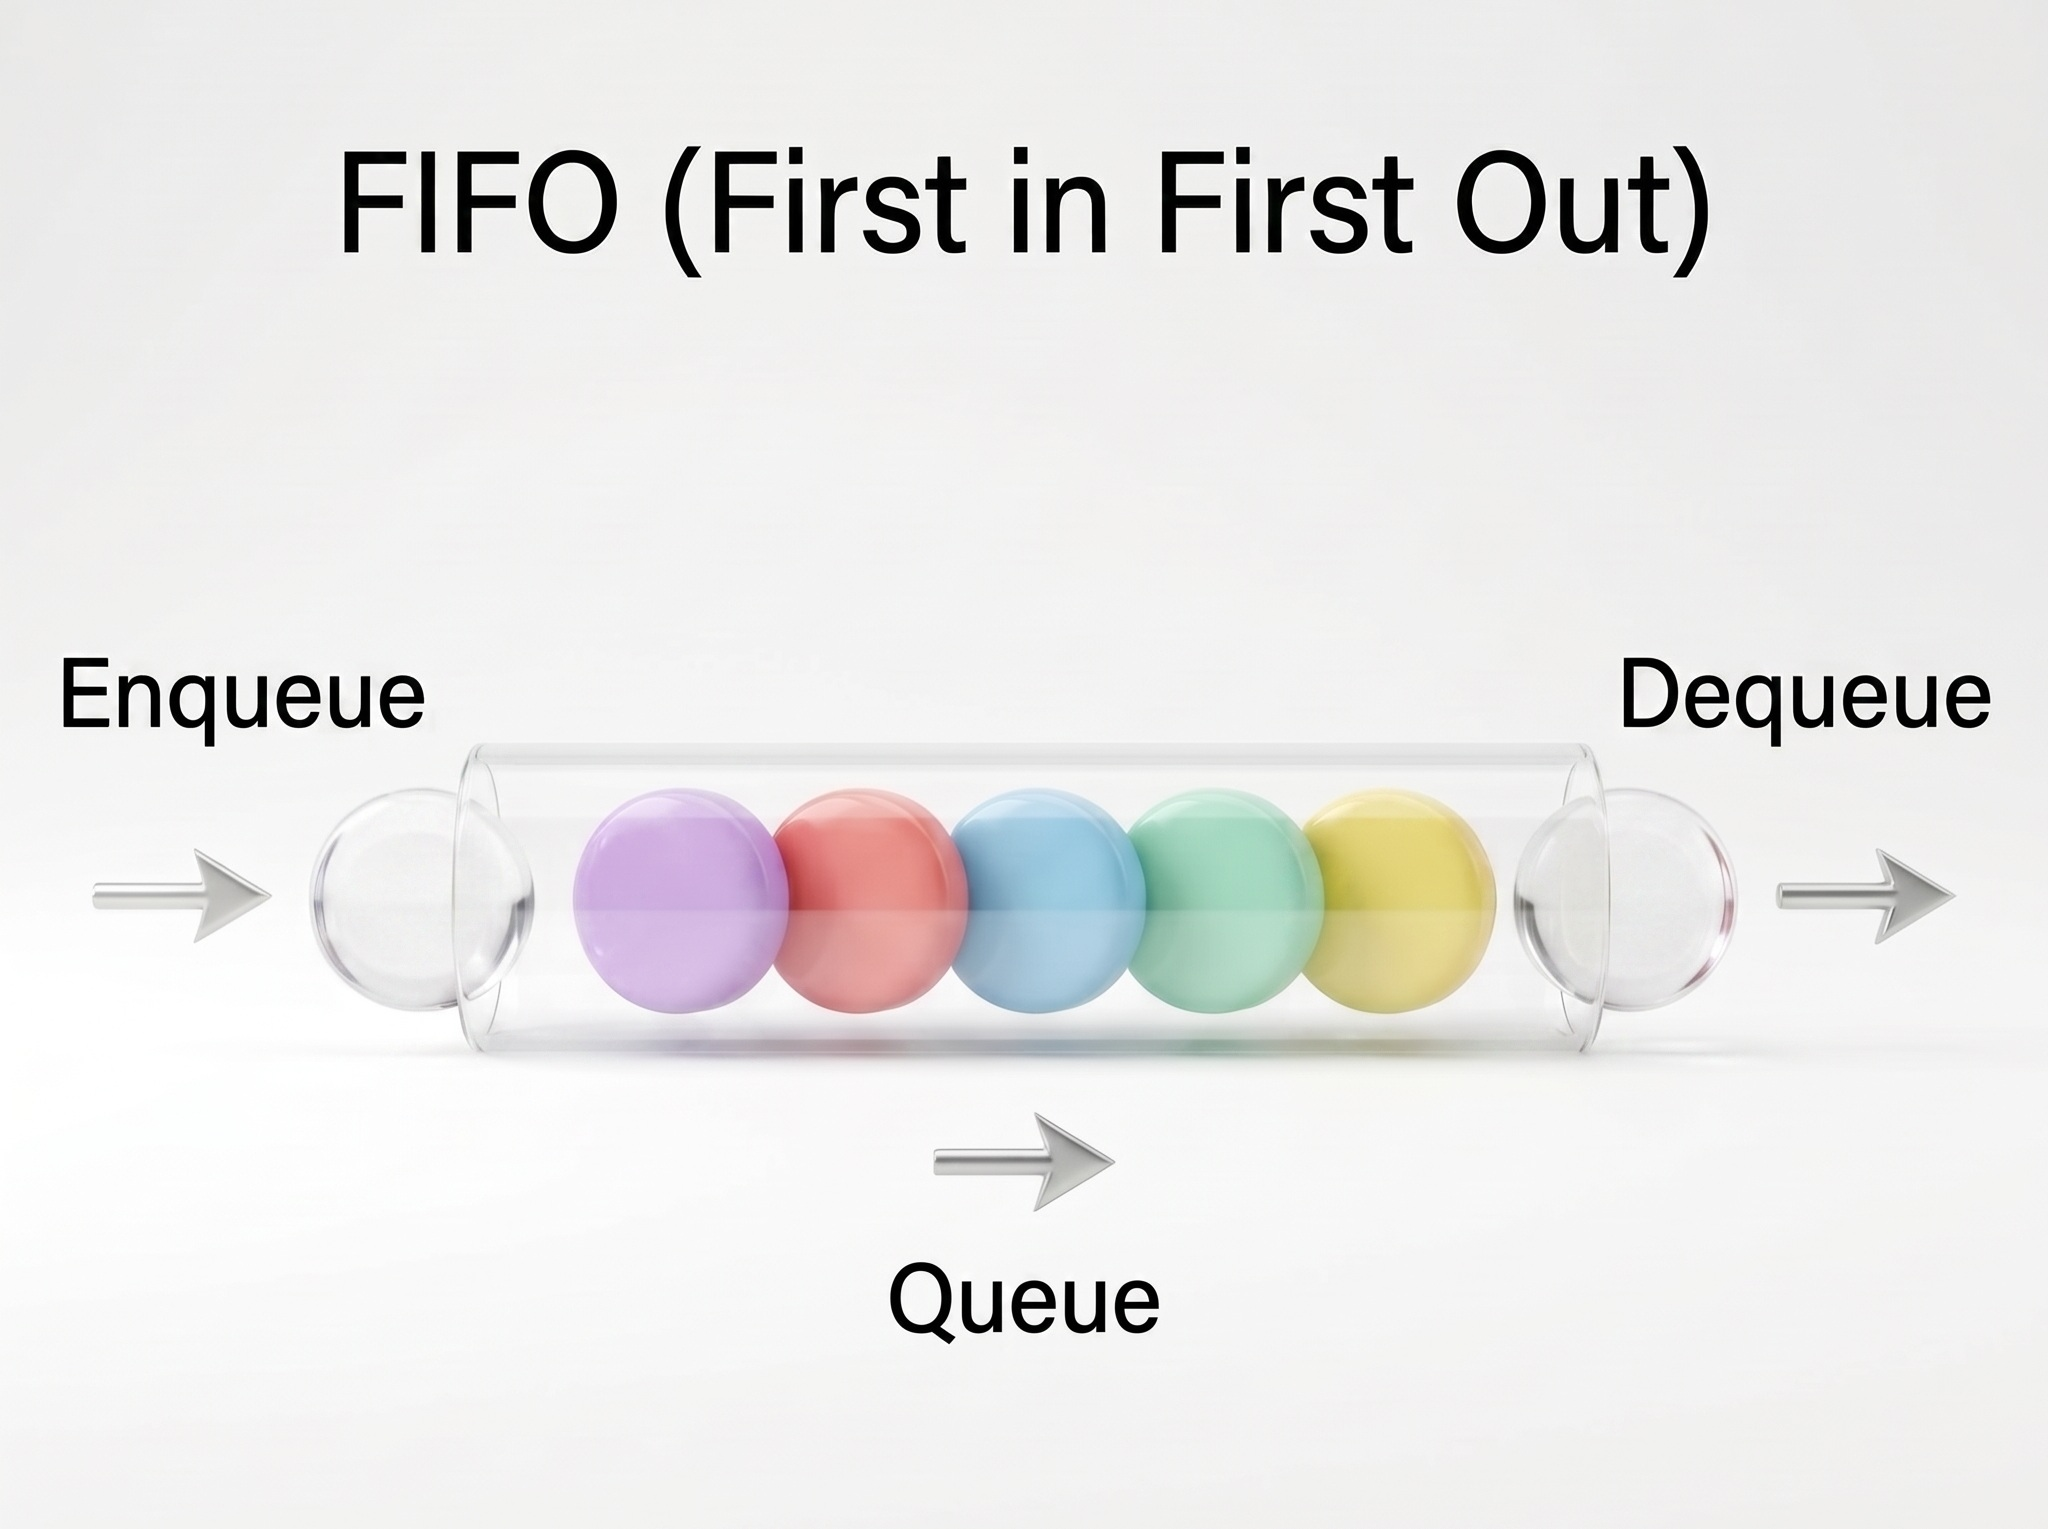
\includegraphics[keepaspectratio,alt={FIFO queue}]{docs/fifo_queue.jpg}}

A FIFO (First-In, First-Out) is a hardware data buffer where the first
piece of data written into the memory is the first piece of data read
out, acting like a queue. An \textbf{asynchronous} FIFO has independent
clocks for writing and reading, allowing systems operating at different
speeds to communicate.

\subsubsection{Why Asynchronous FIFOs
Matter}\label{why-asynchronous-fifos-matter}

Modern digital chips operate different modules with independent clock
frequencies. Asynchronous FIFOs serve as critical data bridges between
these clock domains, ensuring fast and reliable data transfer without
data loss or corruption.

\subsubsection{Project Directory
Structure}\label{project-directory-structure}

{\def\LTcaptype{none} % do not increment counter
\begin{longtable}[]{@{}p{0.18\linewidth}p{0.25\linewidth}p{0.51\linewidth}@{}}
\toprule\noalign{}
Directory & Language / Environment & Purpose \& Key Contents \\
\midrule\noalign{}
\endhead
\bottomrule\noalign{}
\endlastfoot
\textbf{\texttt{rtl/}} & VHDL-2008 & Dual-clock FIFO core (\texttt{fifo.vhd}), memory array, Gray pointers, and 2FF synchronizers \\
\textbf{\texttt{uvm/}} & SystemVerilog (UVM 1.2) & Complete UVM verification suite (Agents, Drivers, Monitors, Sequences, SVA, Scoreboard) \\
\textbf{\texttt{sim/}} & TCL / PowerShell / Batch & Automated simulation runner scripts (\texttt{run.do}, \texttt{run.ps1}, \texttt{run.bat}) \\
\end{longtable}
}

\begin{center}\rule{0.5\linewidth}{0.5pt}\end{center}

\section{2. FIFO Architecture \&
Functionality}\label{2-fifo-architecture--functionality}

\subsection{Top-Level Architecture}\label{top-level-architecture}

\pandocbounded{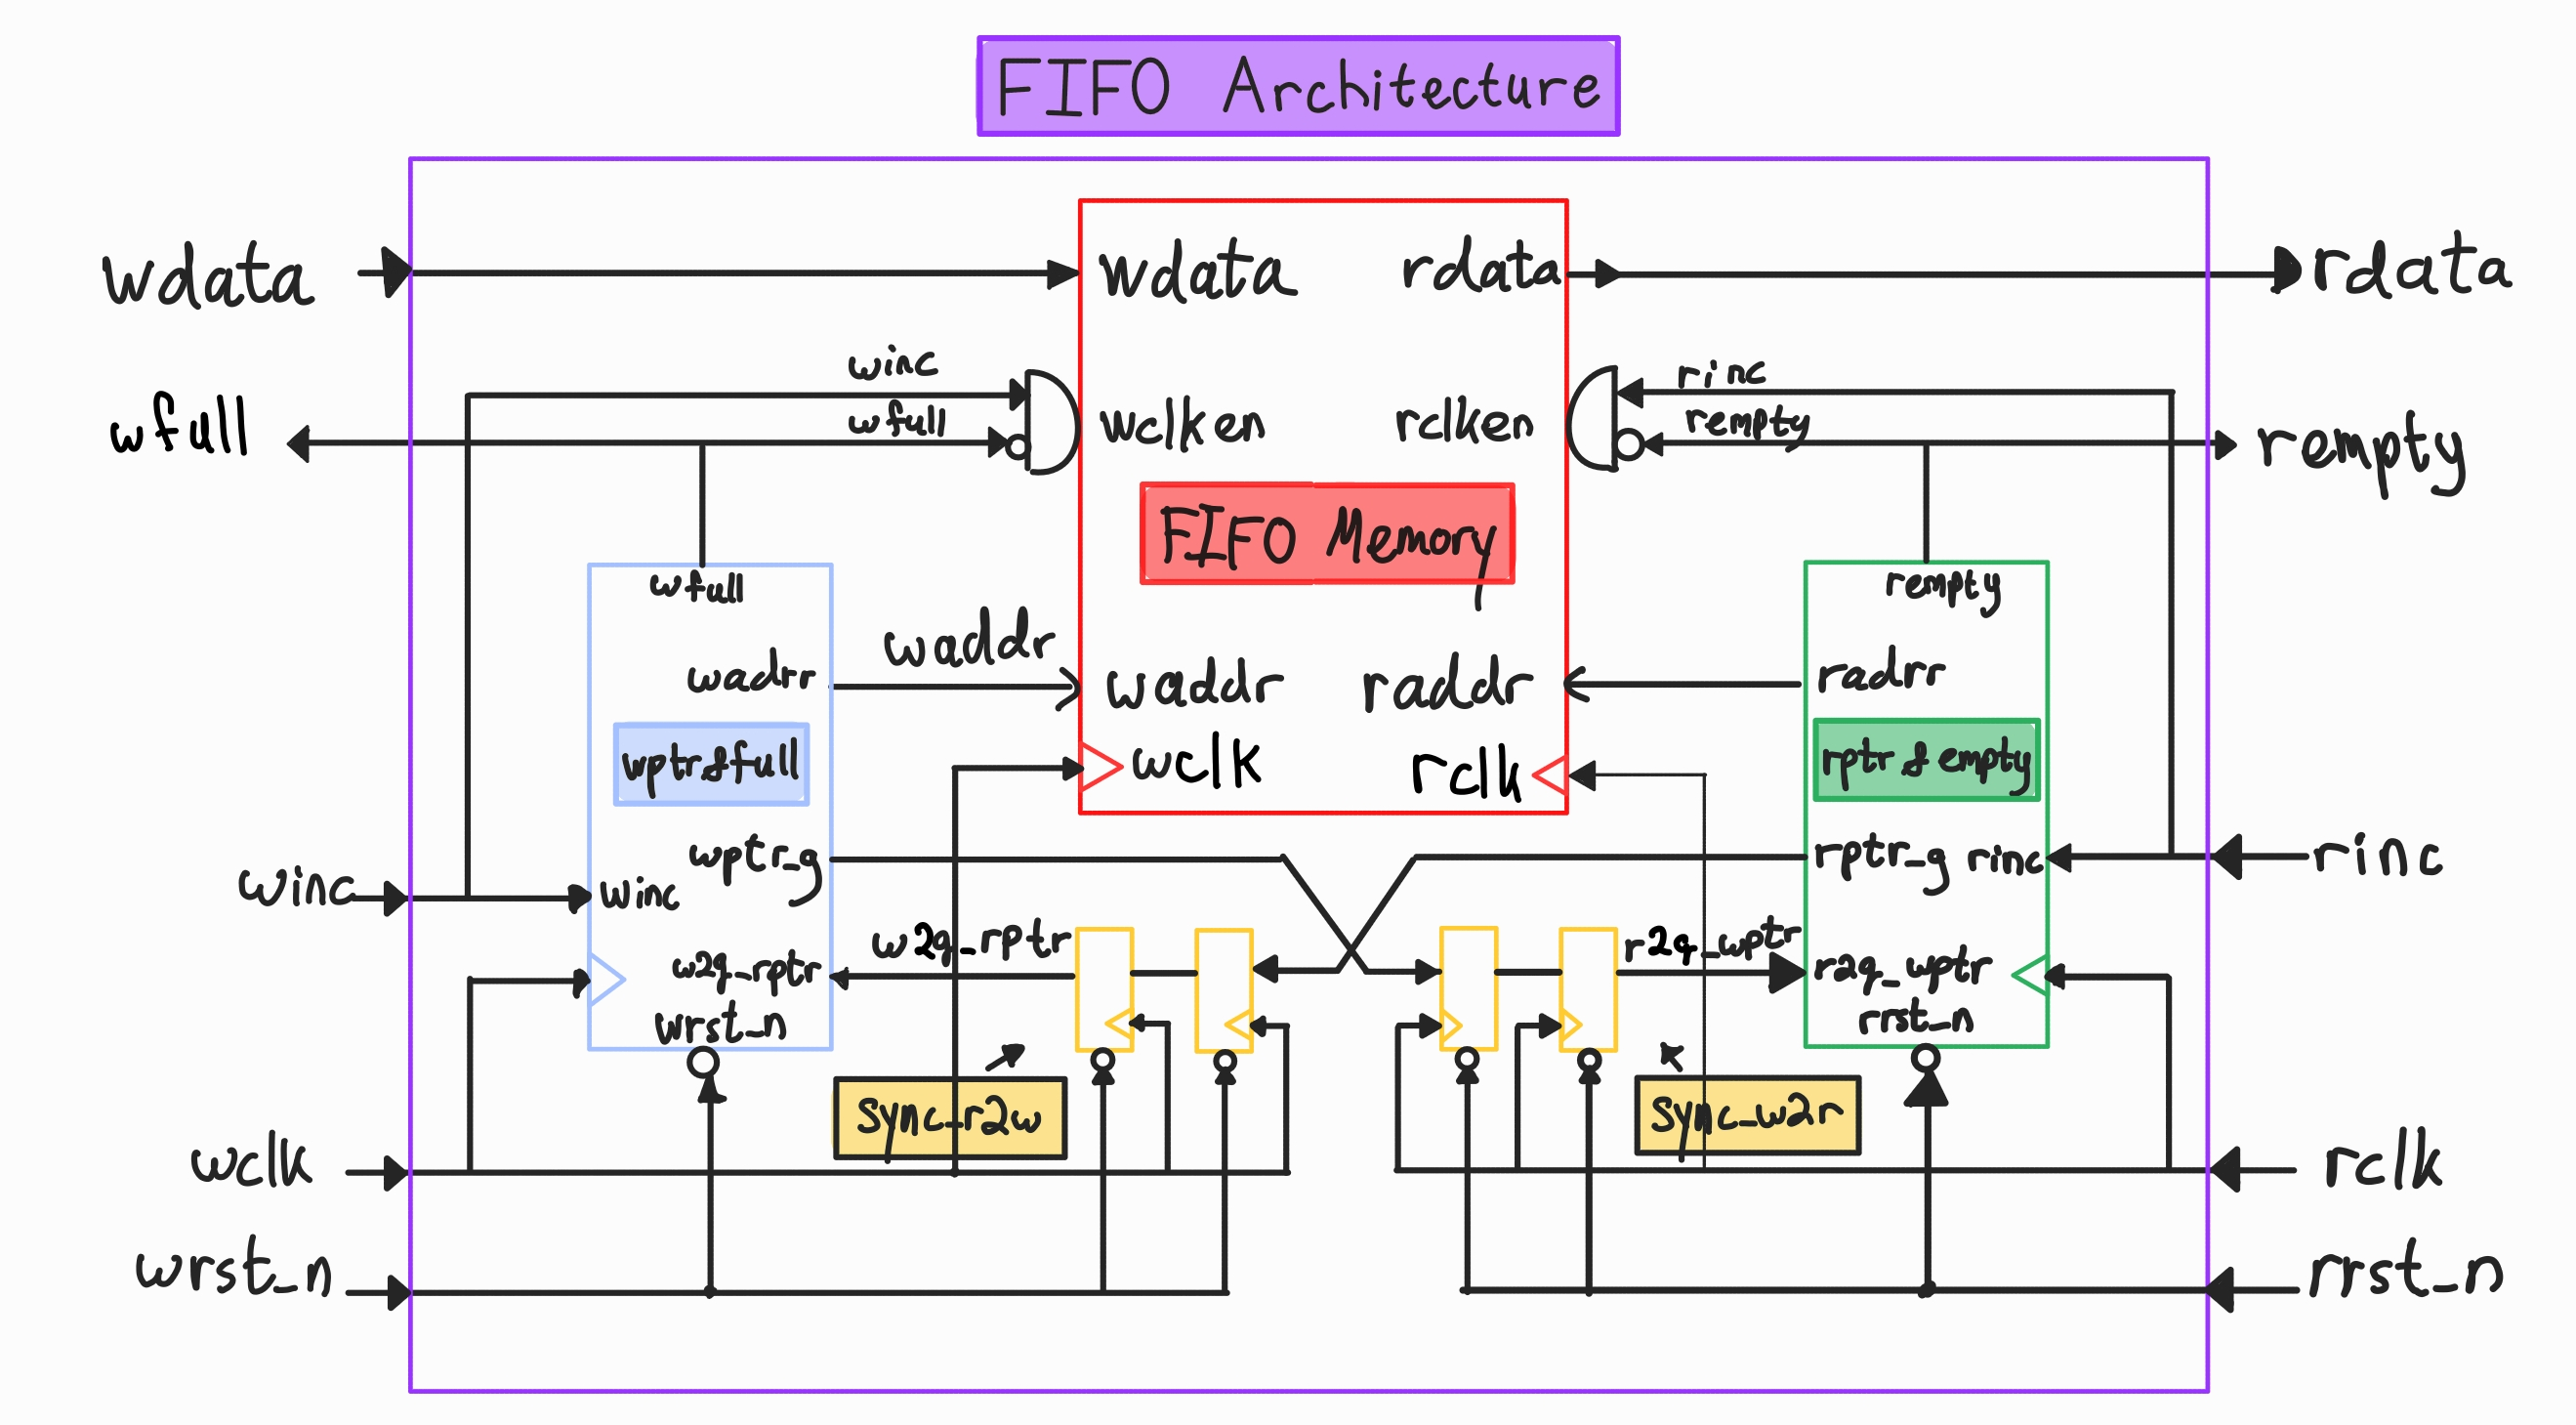
\includegraphics[keepaspectratio,alt={FIFO Architecture}]{docs/FIFO_Block_Diagram.jpg}}

\subsubsection{How the FIFO Works}\label{how-the-fifo-works}

An asynchronous FIFO acts as a temporary queue for transferring data
between two independent clock domains (Write domain and Read domain):

\begin{enumerate}
\def\labelenumi{\arabic{enumi}.}
\tightlist
\item
  \textbf{Writing Data:} When a write is requested and the buffer is not
  full, data is written into memory at the write address, and the write
  pointer increments.
\item
  \textbf{Reading Data:} When a read is requested and the buffer is not
  empty, data is retrieved from memory at the read address, and the read
  pointer increments.
\item
  \textbf{Full \& Empty Status Flags:}

  \begin{itemize}
  \tightlist
  \item
    \textbf{Empty:} Triggered when the read pointer catches up to the
    synchronized write pointer (all data has been read out).
  \item
    \textbf{Full:} Triggered when the write pointer wraps around and
    catches up to the synchronized read pointer (buffer is completely
    filled).
  \end{itemize}
\item
  \textbf{CDC Pointer Transfer:} Pointers are converted to Gray code and
  passed through 2-stage flip-flop (2FF) synchronizers, allowing safe
  cross-domain comparison without sampling skew or metastability.
\end{enumerate}

\begin{center}\rule{0.5\linewidth}{0.5pt}\end{center}

\section{3. Clock Domain Crossing (CDC) \& Synchronization
Architecture}\label{3-clock-domain-crossing-cdc--synchronization-architecture}

Asynchronous clock domain crossings (CDC) pose two fundamental hardware
challenges: \textbf{multi-bit pointer skew} and \textbf{metastability}.
Below is a detailed breakdown of how this FIFO design mitigates both
risks: Section 3.1 addresses pointer skew via Gray code encoding, and Section 3.2 resolves metastability via dual-stage flip-flop synchronizers.

\begin{center}\rule{0.5\linewidth}{0.5pt}\end{center}

\subsection{3.1 Gray Code Encoding}\label{31-gray-code-encoding}

\subsubsection{Problem: Multi-Bit Skew
Corruption}\label{problem-multi-bit-skew-corruption}

In a clock domain crossing, transferring multi-bit pointers is dangerous
due to \textbf{wire/routing skew} and differences in path delays.

When a binary pointer increments, multiple bits often change
simultaneously. For example, when a 3-bit binary pointer transitions
from \texttt{3} (\texttt{011}) to \texttt{4} (\texttt{100}), all three
bits must toggle. Due to routing skew, these bit transitions arrive at
destination flip-flops at slightly different times. If the destination
clock samples the pointer mid-transition, it can capture arbitrary
intermediate corrupted values, leading to false full/empty flag
assertions or corrupted pointer logic.

{\def\LTcaptype{none} % do not increment counter
\begin{longtable}[]{@{}p{0.25\linewidth}p{0.25\linewidth}p{0.46\linewidth}@{}}
\toprule\noalign{}
Current Binary State & Next Binary State & Sampled Intermediate
Values \\
\midrule\noalign{}
\endhead
\bottomrule\noalign{}
\endlastfoot
\textbf{\texttt{011}} (3) & \textbf{\texttt{100}} (4) & \texttt{111}
(7), \texttt{000} (0), \texttt{001} (1), \texttt{101} (5), \texttt{110}
(6), \texttt{010} (2) \\
\end{longtable}
}

\subsubsection{Solution: Single-Bit Toggle (Gray
Code)}\label{solution-single-bit-toggle-gray-code}

To guarantee CDC safety, pointer values are converted to \textbf{Gray
Code} prior to domain crossing. In Gray code, consecutive numerical
values differ by \textbf{exactly one bit}.

\[\text{Binary } 3 \rightarrow 4 \quad \Longleftrightarrow \quad \text{Gray } 010 \rightarrow 110\]

Since only a single bit toggles during pointer increment:

\begin{itemize}
\tightlist
\item
  There are \textbf{no multi-bit intermediate or transient states} to
  sample.
\item
  If the receiving clock samples the signal precisely during a bit
  transition, the sampled result will resolve to either the
  \textbf{previous state} (\texttt{010}) or the \textbf{new state}
  (\texttt{110}).
\item
  Both are valid, coherent pointer states. Sampling the old value simply
  delays flag assertion by one destination clock cycle (safe pessimism)
  without corrupting memory management logic.
\end{itemize}

\subsubsection{Implementation: Binary-to-Gray
Converter}\label{implementation-binary-to-gray-converter}

\[\text{G} = \text{B} \text{ xor } (\text{B} \gg 1)\]

\begin{center}\rule{0.5\linewidth}{0.5pt}\end{center}

\subsection{3.2 Preventing Metastability
(Synchronizers)}\label{32-preventing-metastability-synchronizers}

\subsubsection{Problem: Setup/Hold Timing
Violations}\label{problem-setuphold-timing-violations}

Even with Gray-coded pointers, a single transitioning bit can still
violate the setup or hold timing requirements of the receiving
flip-flop, leading to \textbf{metastability}.

Flip-flops require input signals to remain stable during a setup and
hold window around the active clock edge. Because the clocks are
asynchronous, such violations cannot be completely avoided.

\paragraph{How Metastability Occurs --- Internal Flip-Flop
Dynamics}\label{how-metastability-occurs--internal-flip-flop-dynamics}

A flip-flop can be viewed internally as a regenerative circuit
containing cross-coupled inverters controlled by transmission gates.

\begin{enumerate}
\def\labelenumi{\arabic{enumi}.}
\item
  \textbf{Before the Clock Edge:} The input data propagates through the
  input stage and establishes a voltage on an internal storage node.\\
  \pandocbounded{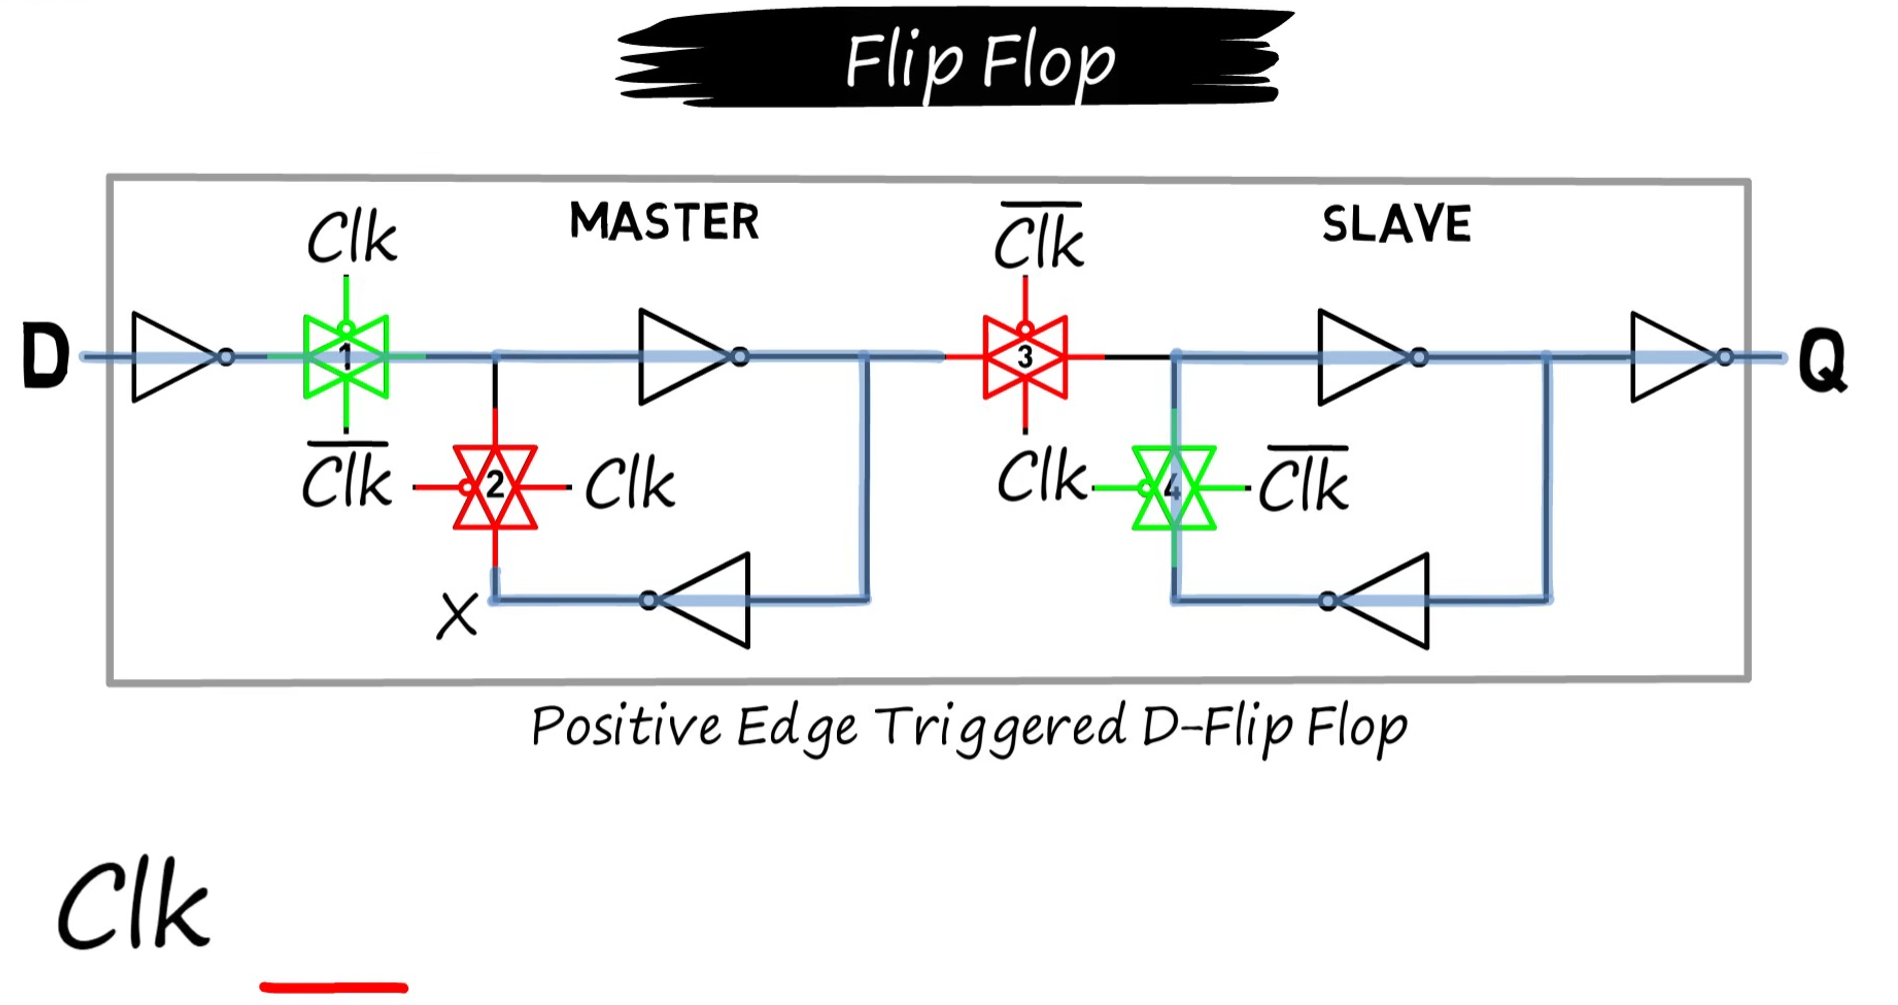
\includegraphics[keepaspectratio,alt={Before Edge}]{docs/Before_Edge.png}}
\item
  \textbf{At the Clock Edge:} The transmission gates change state,
  disconnecting the input path and enabling the regenerative feedback
  path. If the input changes within the setup/hold window, the internal
  nodes may contain conflicting voltage levels.\\
  \pandocbounded{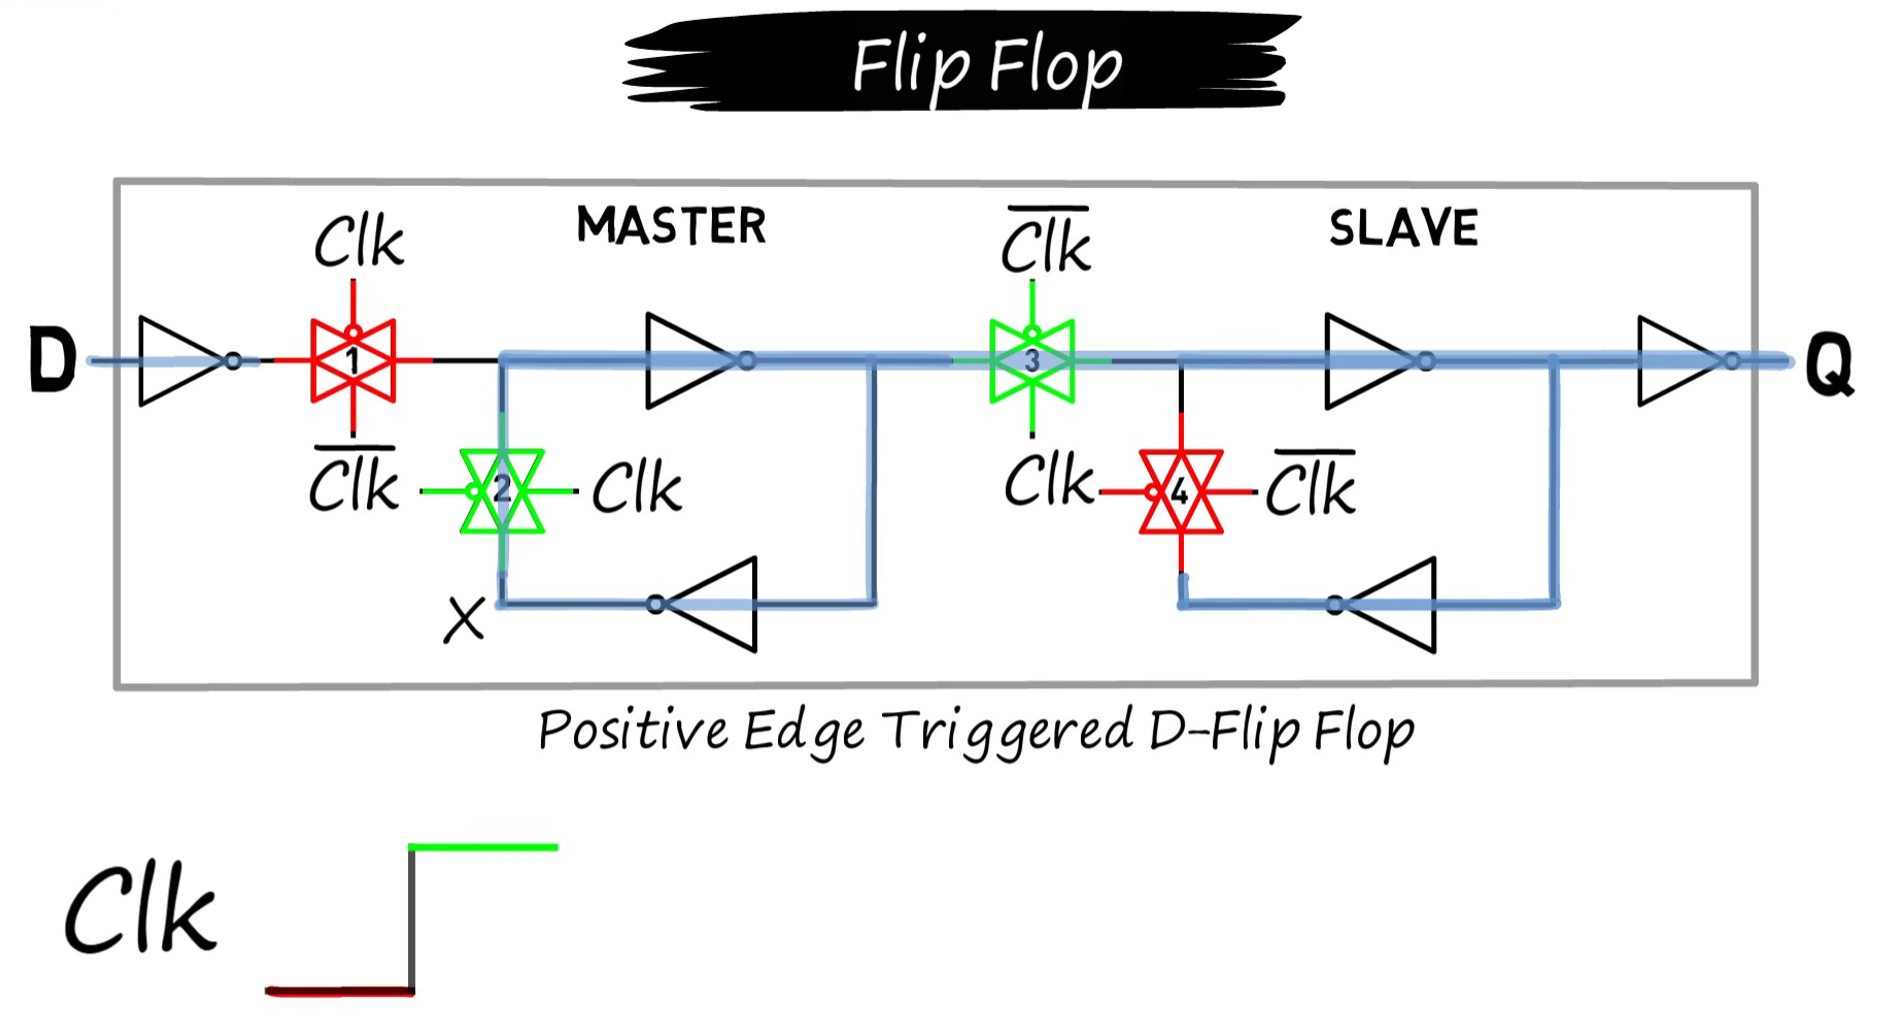
\includegraphics[keepaspectratio,alt={After Edge}]{docs/After_Edge.png}}
\item
  \textbf{Analog Contention:} At this point, the internal nodes are no
  longer behaving as ideal digital 0/1 signals. The feedback path and
  the transmission-gate paths interact dynamically. One node can drive
  the other through the feedback inverters while the other node
  simultaneously affects the first. The exact transient behavior depends
  on transistor drive strengths, capacitances, propagation delays, and
  process variations.\\
  \pandocbounded{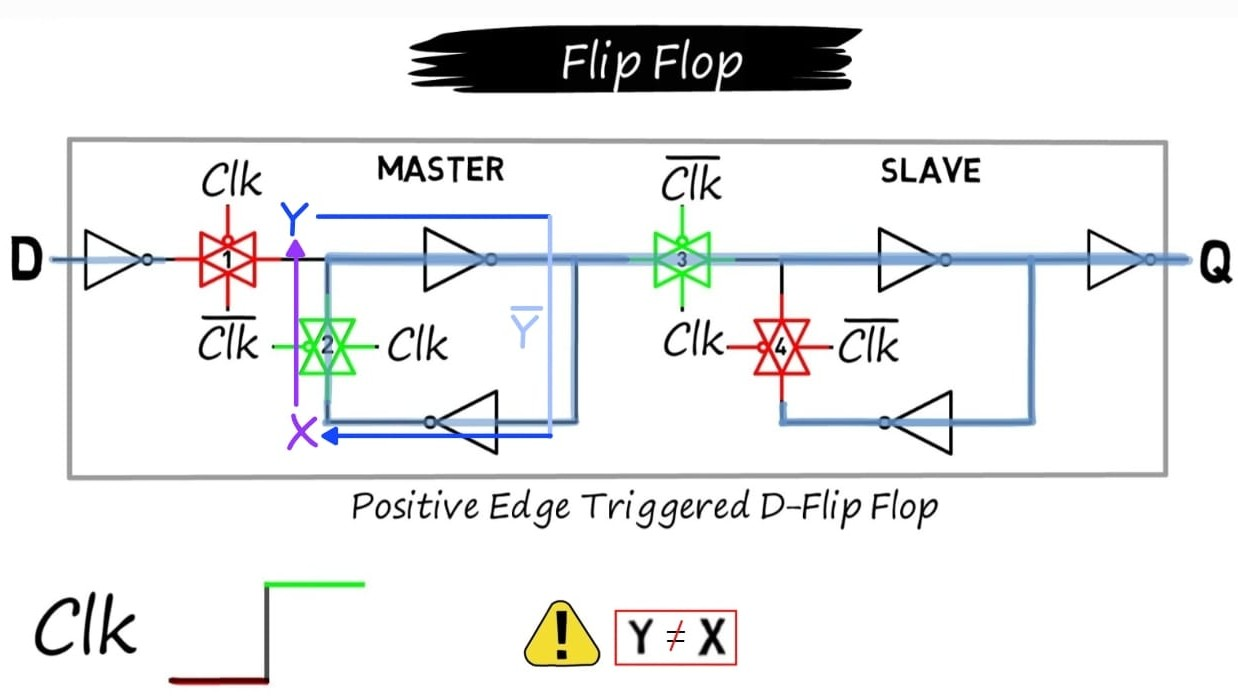
\includegraphics[keepaspectratio,alt={Metastable state}]{docs/Metastable_state.jpeg}}
\item
  \textbf{Metastable Equilibrium:} The cross-coupled inverter pair has
  two stable states (logic 0 and logic 1) and an unstable equilibrium
  point between them. This equilibrium voltage, often denoted \(V_M\),
  is typically near \(V_{DD}/2\), but is not necessarily exactly
  \(V_{DD}/2\).

  If the contention leaves the regenerative loop sufficiently close to
  this unstable equilibrium, the positive feedback initially has only a
  very small voltage difference to amplify. The circuit therefore
  requires additional time to resolve to a valid logic 0 or 1.
\item
  \textbf{Regeneration:} Around the metastable point, the voltage
  difference can grow approximately exponentially:
\end{enumerate}

\[\Delta V(t) = \Delta V_0 e^{t/\tau}\]

where \(\Delta V_0\) is the initial voltage difference from the
metastable equilibrium and \(\tau\) is the characteristic resolution
time constant of the circuit.

Therefore, the closer the internal state is to the unstable equilibrium
after the initial transient, the longer the resolution can take. The
important quantity is not whether a node is exactly at \(V_{DD}/2\), but
how close the regenerative circuit as a whole is to its unstable
equilibrium.

\begin{enumerate}
\def\labelenumi{\arabic{enumi}.}
\setcounter{enumi}{5}
\item
  \textbf{Setup Violation:} Occurs if input \(D\) transitions too close
  to the clock edge. Although \(D\) propagates through the input
  transmission gate to node \(Y\), it fails to propagate through the
  internal inverters in time to establish a stable, matching voltage on
  node \(X\) before sampling. When the clock edge arrives and the
  feedback transmission gate closes while \(Y \neq X\), the conflicting
  voltages fight each other, trapping the regenerative latch near its
  unstable equilibrium and causing metastability.\\
  \pandocbounded{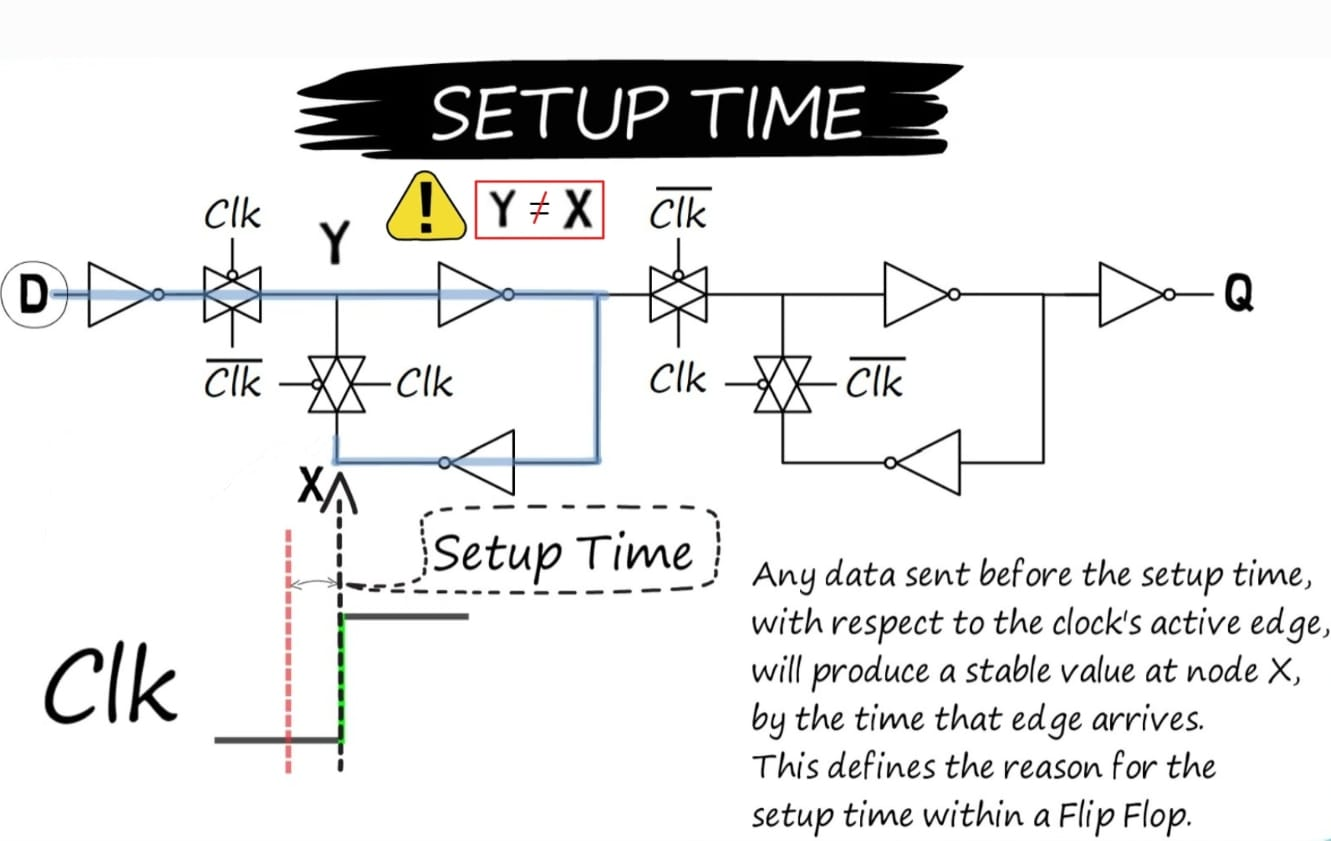
\includegraphics[keepaspectratio,alt={Setup Time Violation}]{docs/Setup_Time.jpeg}}
\item
  \textbf{Hold Violation:} Occurs if input \(D\) changes too soon after
  the clock edge. Because the input transmission gate requires finite
  time to fully shut off, a premature transition on \(D\) leaks into
  node \(Y\) while the feedback transmission gate is already closing.
  This disrupts the closing feedback loop (\(Y \neq X\)), disturbing the
  settling state and potentially forcing the regenerative latch back
  toward metastability.\\
  \pandocbounded{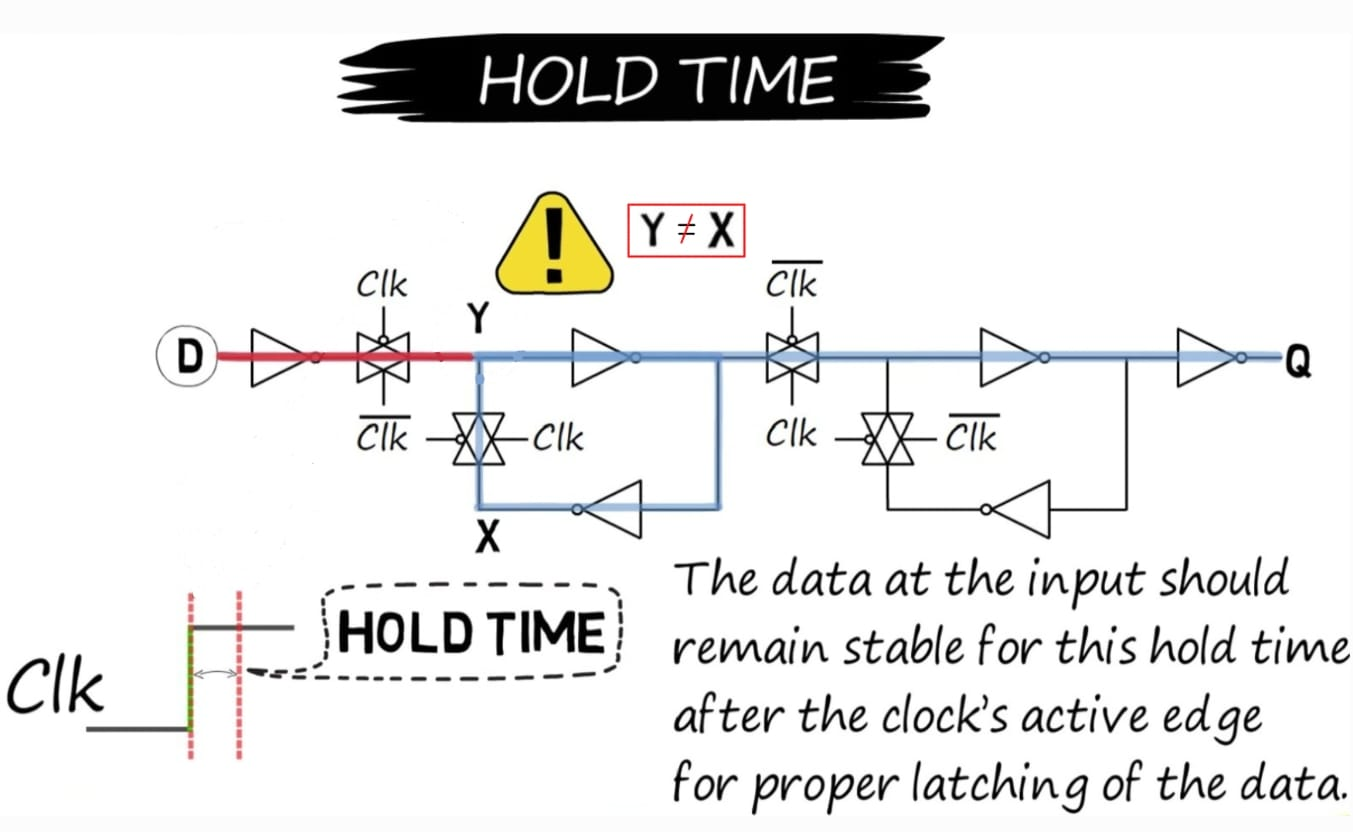
\includegraphics[keepaspectratio,alt={Hold Time Violation}]{docs/Hold_Time.jpeg}}
\end{enumerate}

\paragraph{Key Point}\label{key-point}

Metastability occurs when a timing violation leaves internal nodes in
conflict (\(Y \neq X\)), closing the regenerative feedback loop forces
the latch close to its unstable equilibrium point (\(V_M\)). The closer
the initial voltage difference (\(\Delta V_0\)) is to zero, the longer
positive feedback requires to amplify the signal and resolve the
flip-flop to a valid digital \textquotesingle0\textquotesingle{} or
\textquotesingle1\textquotesingle.

\begin{center}\rule{0.5\linewidth}{0.5pt}\end{center}

\subsubsection{Solution: Synchronizers
(2FF)}\label{solution-synchronizers-2ff}

To prevent metastable outputs from propagating into internal control
logic, Gray-coded pointers pass through \textbf{2-Stage Flip-Flop
Chains} granting a full clock cycle of resolution time for any
metastable state to decay

\pandocbounded{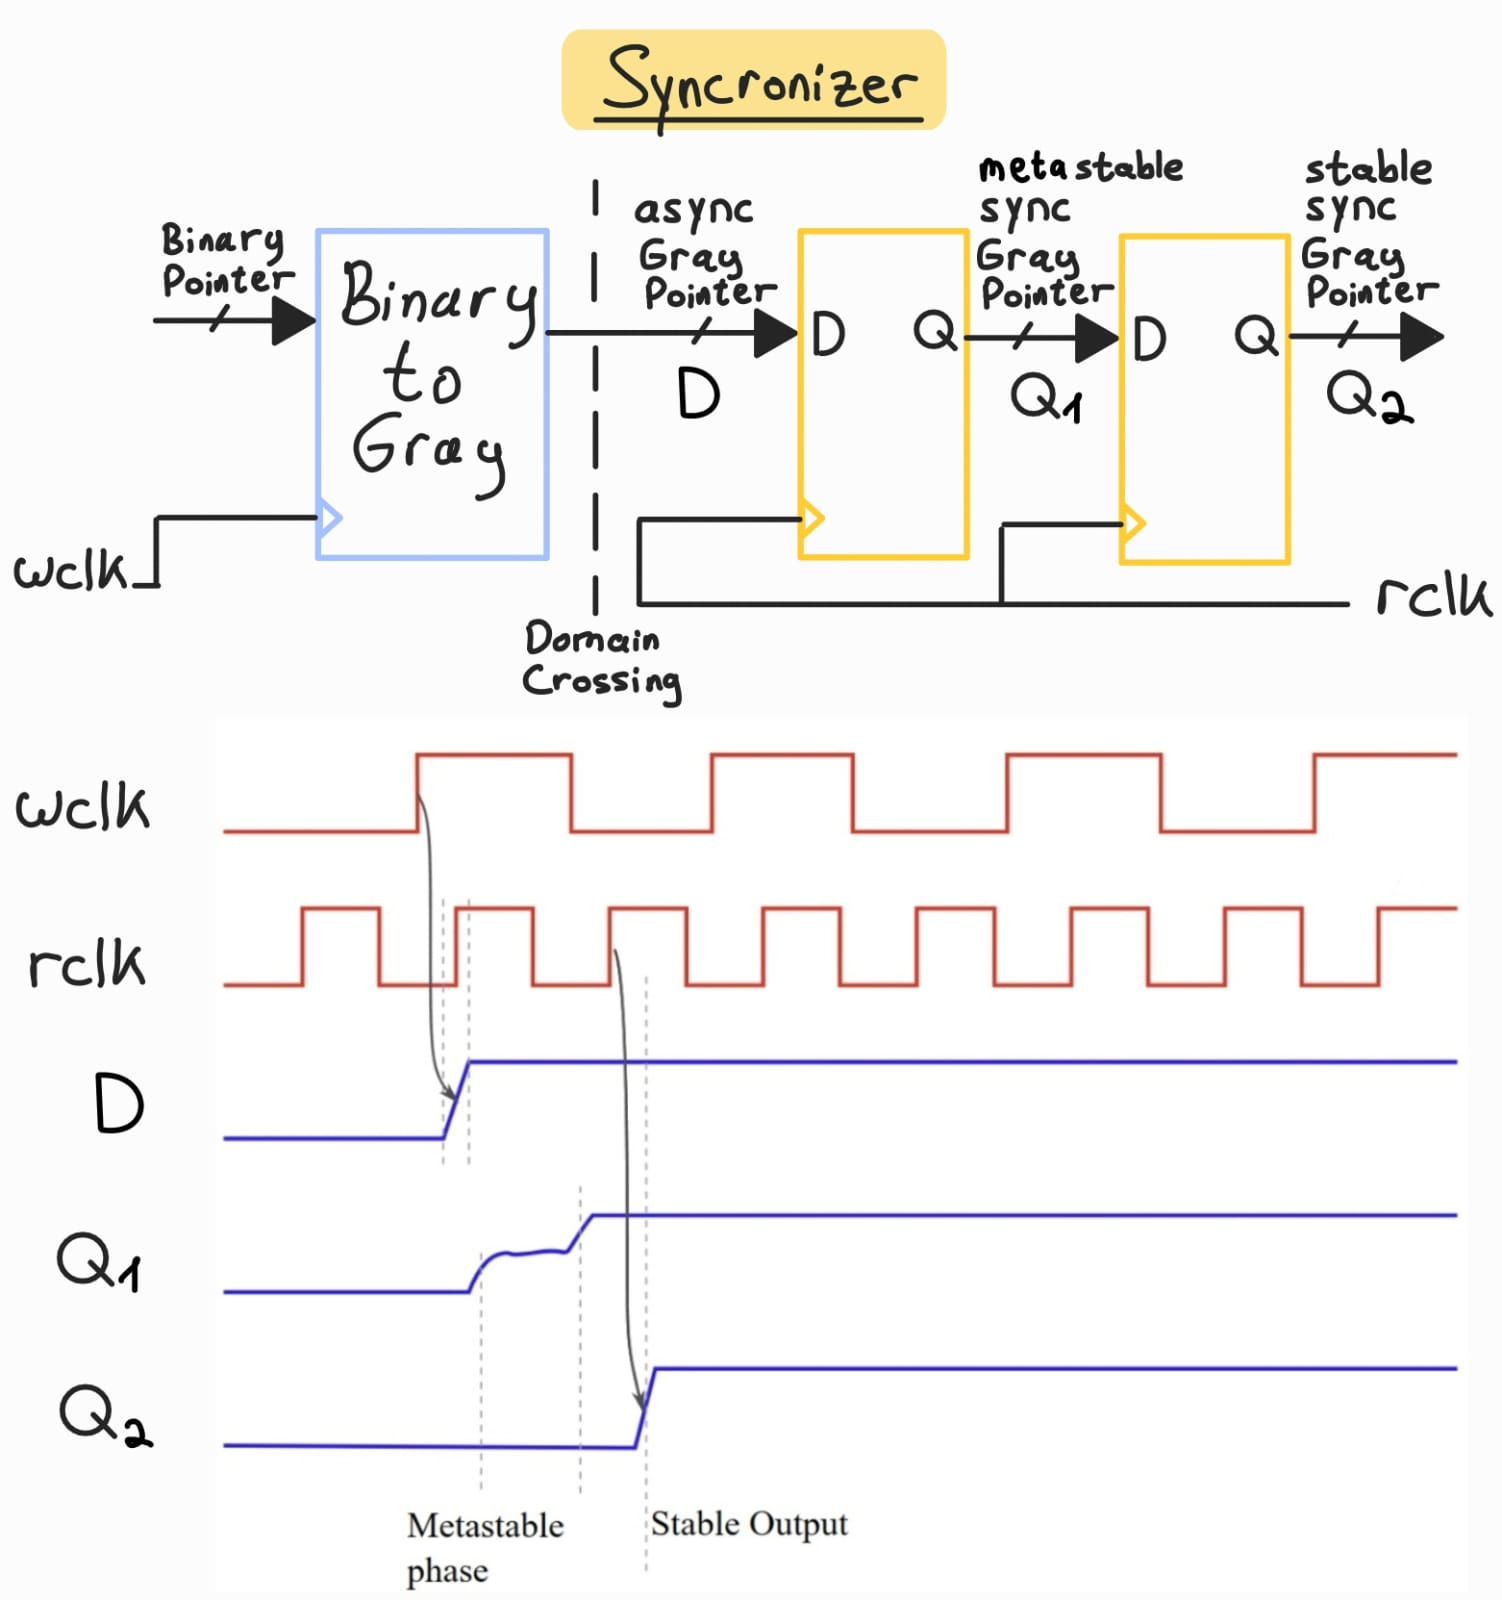
\includegraphics[keepaspectratio,alt={2FF Synchronizer Architecture}]{docs/Gray_Pointer_Syncronizer.jpeg}}

\begin{enumerate}
\def\labelenumi{\arabic{enumi}.}
\tightlist
\item
  \textbf{Stage 1 (\(Q_1\)):} Samples the raw asynchronous Gray pointer.
  If a setup/hold violation occurs, \(Q_1\) may become metastable.
\item
  \textbf{Resolution Window (\(t_r\)):} \(Q_1\) is given approximately
  one destination-clock cycle for any metastable condition to resolve
  through the regenerative feedback into a deterministic digital
  \textquotesingle0\textquotesingle{} or
  \textquotesingle1\textquotesingle.
\item
  \textbf{Stage 2 (\(Q_2\)):} Samples the settled output of \(Q_1\).
  Because the probability of \(Q_1\) remaining metastable for a full
  clock cycle is exponentially low, \(Q_2\) creates a clean,
  synchronized signal.
\end{enumerate}

\paragraph{Mean Time Between Failures
(MTBF)}\label{mean-time-between-failures-mtbf}

The reliability of a synchronizer chain is quantified by its MTBF, which
increases exponentially with the resolution time (\(t_r\)):

\[\text{MTBF} = \frac{e^{s \cdot t_r}}{T_0 \cdot f_{\text{clk}} \cdot f_{\text{data}}}\]

{\def\LTcaptype{none} % do not increment counter
\begin{longtable}[]{@{}p{0.25\linewidth}p{0.71\linewidth}@{}}
\toprule\noalign{}
Parameter & Description \\
\midrule\noalign{}
\endhead
\bottomrule\noalign{}
\endlastfoot
\textbf{\(t_r\)} & Available settling time
(\(T_{\text{clk}} - t_{su}\)) \\
\textbf{\(s\)} & Resolution time constant of the process node \\
\textbf{\(T_0\)} & Deep-metastability aperture factor \\
\textbf{\(f_{\text{clk}}\) / \(f_{\text{data}}\)} & Destination clock
frequency and incoming Gray pointer toggle rate \\
\end{longtable}
}

The insertion of \(Q_2\) expands \(t_r\) by nearly an entire clock
period, which can boost MTBF from seconds to years.

\begin{center}\rule{0.5\linewidth}{0.5pt}\end{center}

\subsection{3.3 Synchronization Latency \& Safe Flag
Pessimism}\label{33-synchronization-latency--safe-flag-pessimism}

Passing pointers across asynchronous clock domains via 2FF synchronizers
introduces a \textbf{2 clock cycle delay}. Because pointers are compared
against slightly delayed values from the opposite domain, status flags
operate with a \textbf{safe, pessimistic bias}:

\begin{itemize}
\item
  \textbf{\texttt{wfull} Pessimism:} Compares write pointer to a read
  pointer that is 2 cycles old. The write domain may see the FIFO as
  "Full" slightly longer than it actually is (if reads occurred during
  synchronization).

  \begin{itemize}
  \tightlist
  \item
    \textbf{Safety Impact:} Prevents \textbf{overflow} (overwriting
    data), at the cost of a temporary pause in write throughput.
  \end{itemize}
\item
  \textbf{\texttt{rempty} Pessimism:} Compares read pointer to a write
  pointer that is 2 cycles old. The read domain may see the FIFO as
  "Empty" slightly longer than it actually is (if writes occurred during
  synchronization).

  \begin{itemize}
  \tightlist
  \item
    \textbf{Safety Impact:} Prevents \textbf{underflow} (reading garbage
    data), at the cost of a 2-cycle latency delay before newly written
    data can be read out.
  \end{itemize}
\end{itemize}

\begin{center}\rule{0.5\linewidth}{0.5pt}\end{center}

\section{4. UVM Verification
Environment}\label{4-uvm-verification-environment}

\subsection{Why a Simple Testbench is
Insufficient}\label{why-a-simple-testbench-is-insufficient}

A standard testbench focuses on toggling individual pins, making it
difficult to handle the multiple clock domains and unpredictable timing
of an asynchronous FIFO. To avoid debugging race conditions in the test
code itself, we use SystemVerilog UVM to elevate the abstraction from
"wiggling pins" to "sending transactions".

\subsubsection{The Core Advantages of
UVM:}\label{the-core-advantages-of-uvm}

\begin{enumerate}
\def\labelenumi{\arabic{enumi}.}
\tightlist
\item
  \textbf{Modularity:} UVM strictly isolates data generation, pin
  driving, and result checking into different components. This allows us
  to easily change one component without affecting the others.
\item
  \textbf{Standardized Communication:} UVM libraries provide Transaction
  Level Modeling (TLM). Standardizing communication guarantees data is
  passed safely between testbench components without race conditions.
\item
  \textbf{Scalability:} Scaling vertically or horizontally is trivial.
  We can easily add more FIFOs into the same testing enviroment by
  copying the agents and connecting them to the new fifo. Alternatively,
  we can integrate this FIFO into a larger SoC, by plugging the
  testbench into a larger verification environment without modification.
\end{enumerate}

\begin{center}\rule{0.5\linewidth}{0.5pt}\end{center}

\subsection{UVM Testbench
Architecture}\label{uvm-testbench-architecture}

\pandocbounded{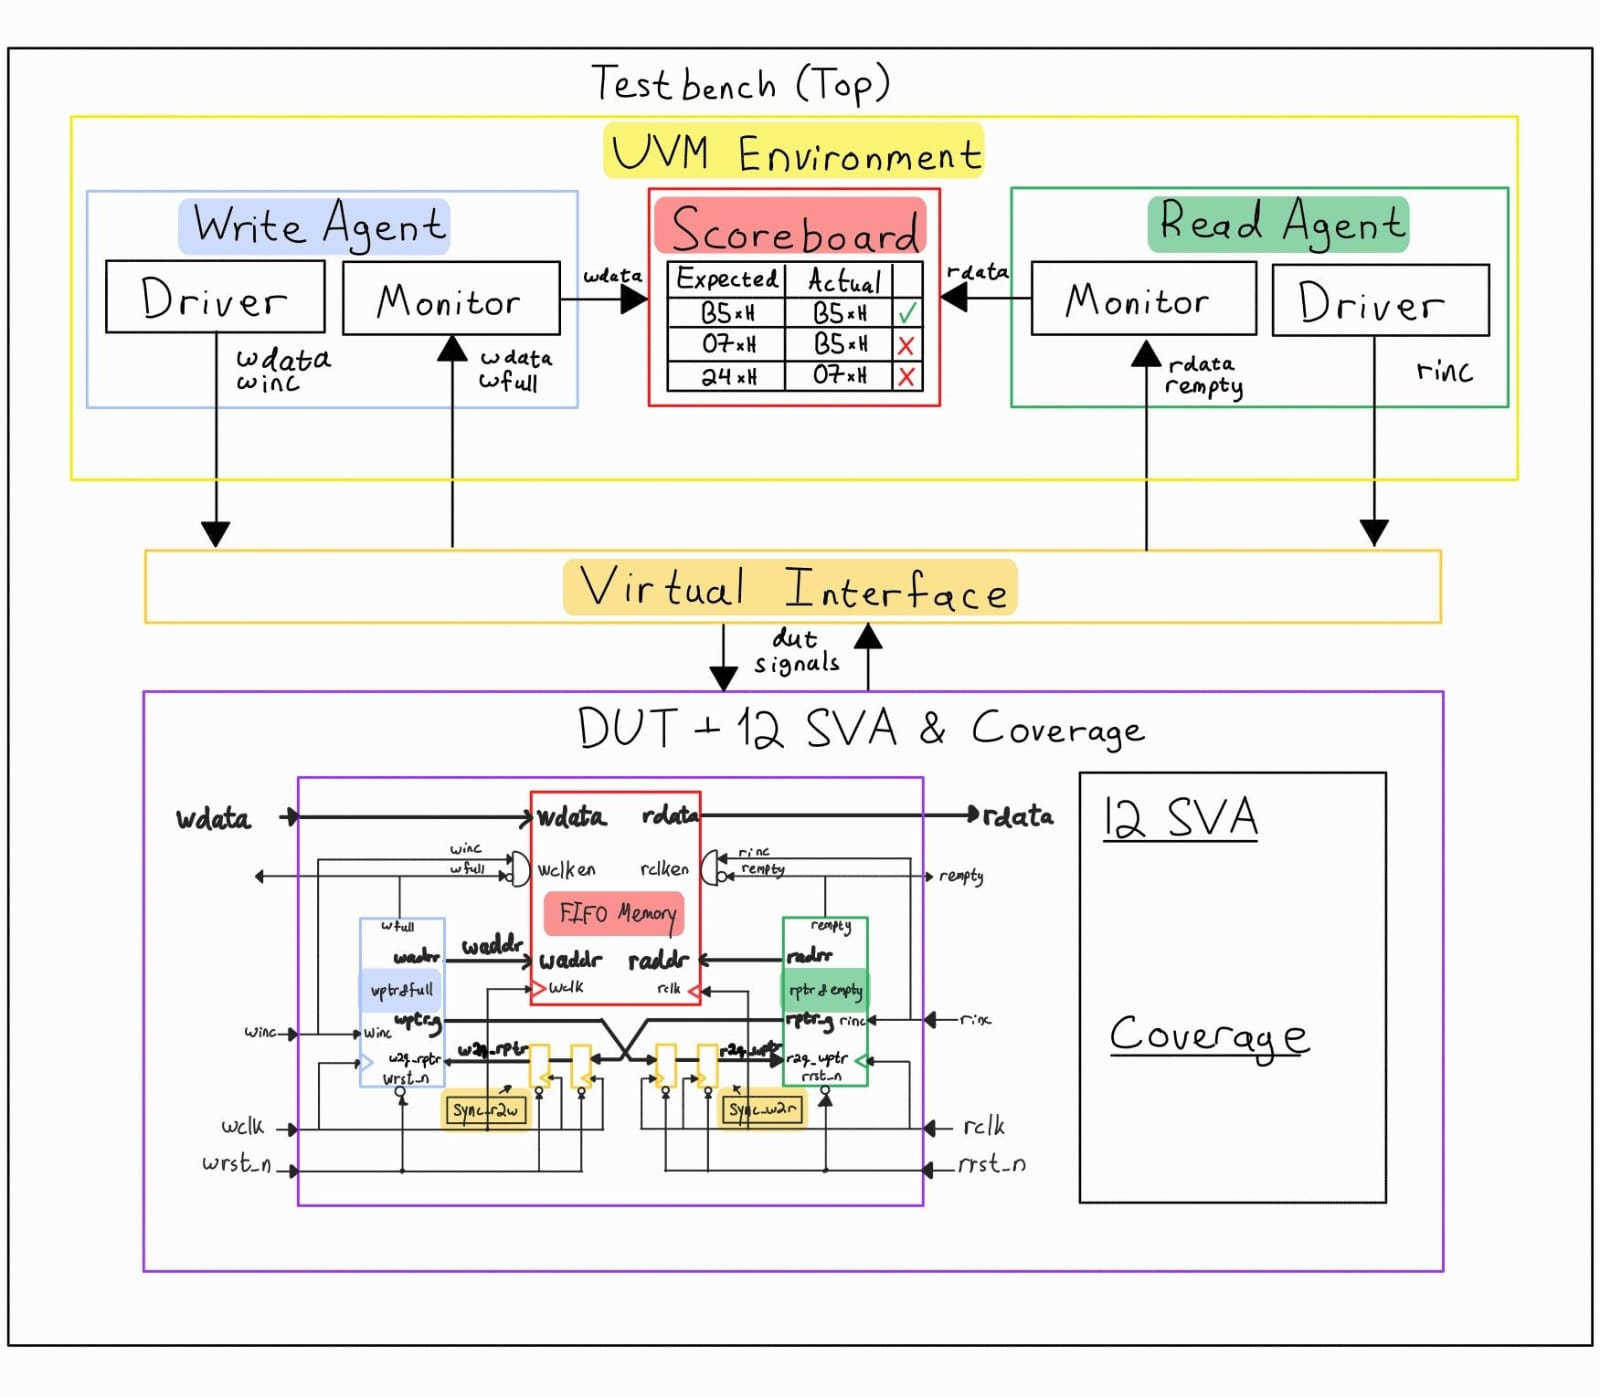
\includegraphics[keepaspectratio,alt={UVM Testbench Architecture}]{docs/UVM_Architecture.jpeg}}

The testbench operates using five primary UVM components:

\begin{itemize}
\tightlist
\item
  \textbf{Agents:} The managers of a specific clock domain. They
  encapsulate the data generation, driving, and monitoring activity for
  their respective sides of the FIFO.
\item
  \textbf{Drivers:} Drive DUT input signals.
\item
  \textbf{Monitors:} Monitor hardware signals and send them to the
  scoreboard.
\item
  \textbf{Scoreboard:} Records data pushed into the FIFO and compares it
  against data popped out to verify zero data corruption.
\item
  \textbf{Virtual Interface:} Allows the testbench to drive and monitor
  signals on the DUT\textquotesingle s pins.
\end{itemize}

\subsubsection{[Transport] UVM Logistics
Analogy}\label{truck-uvm-logistics-analogy}

\pandocbounded{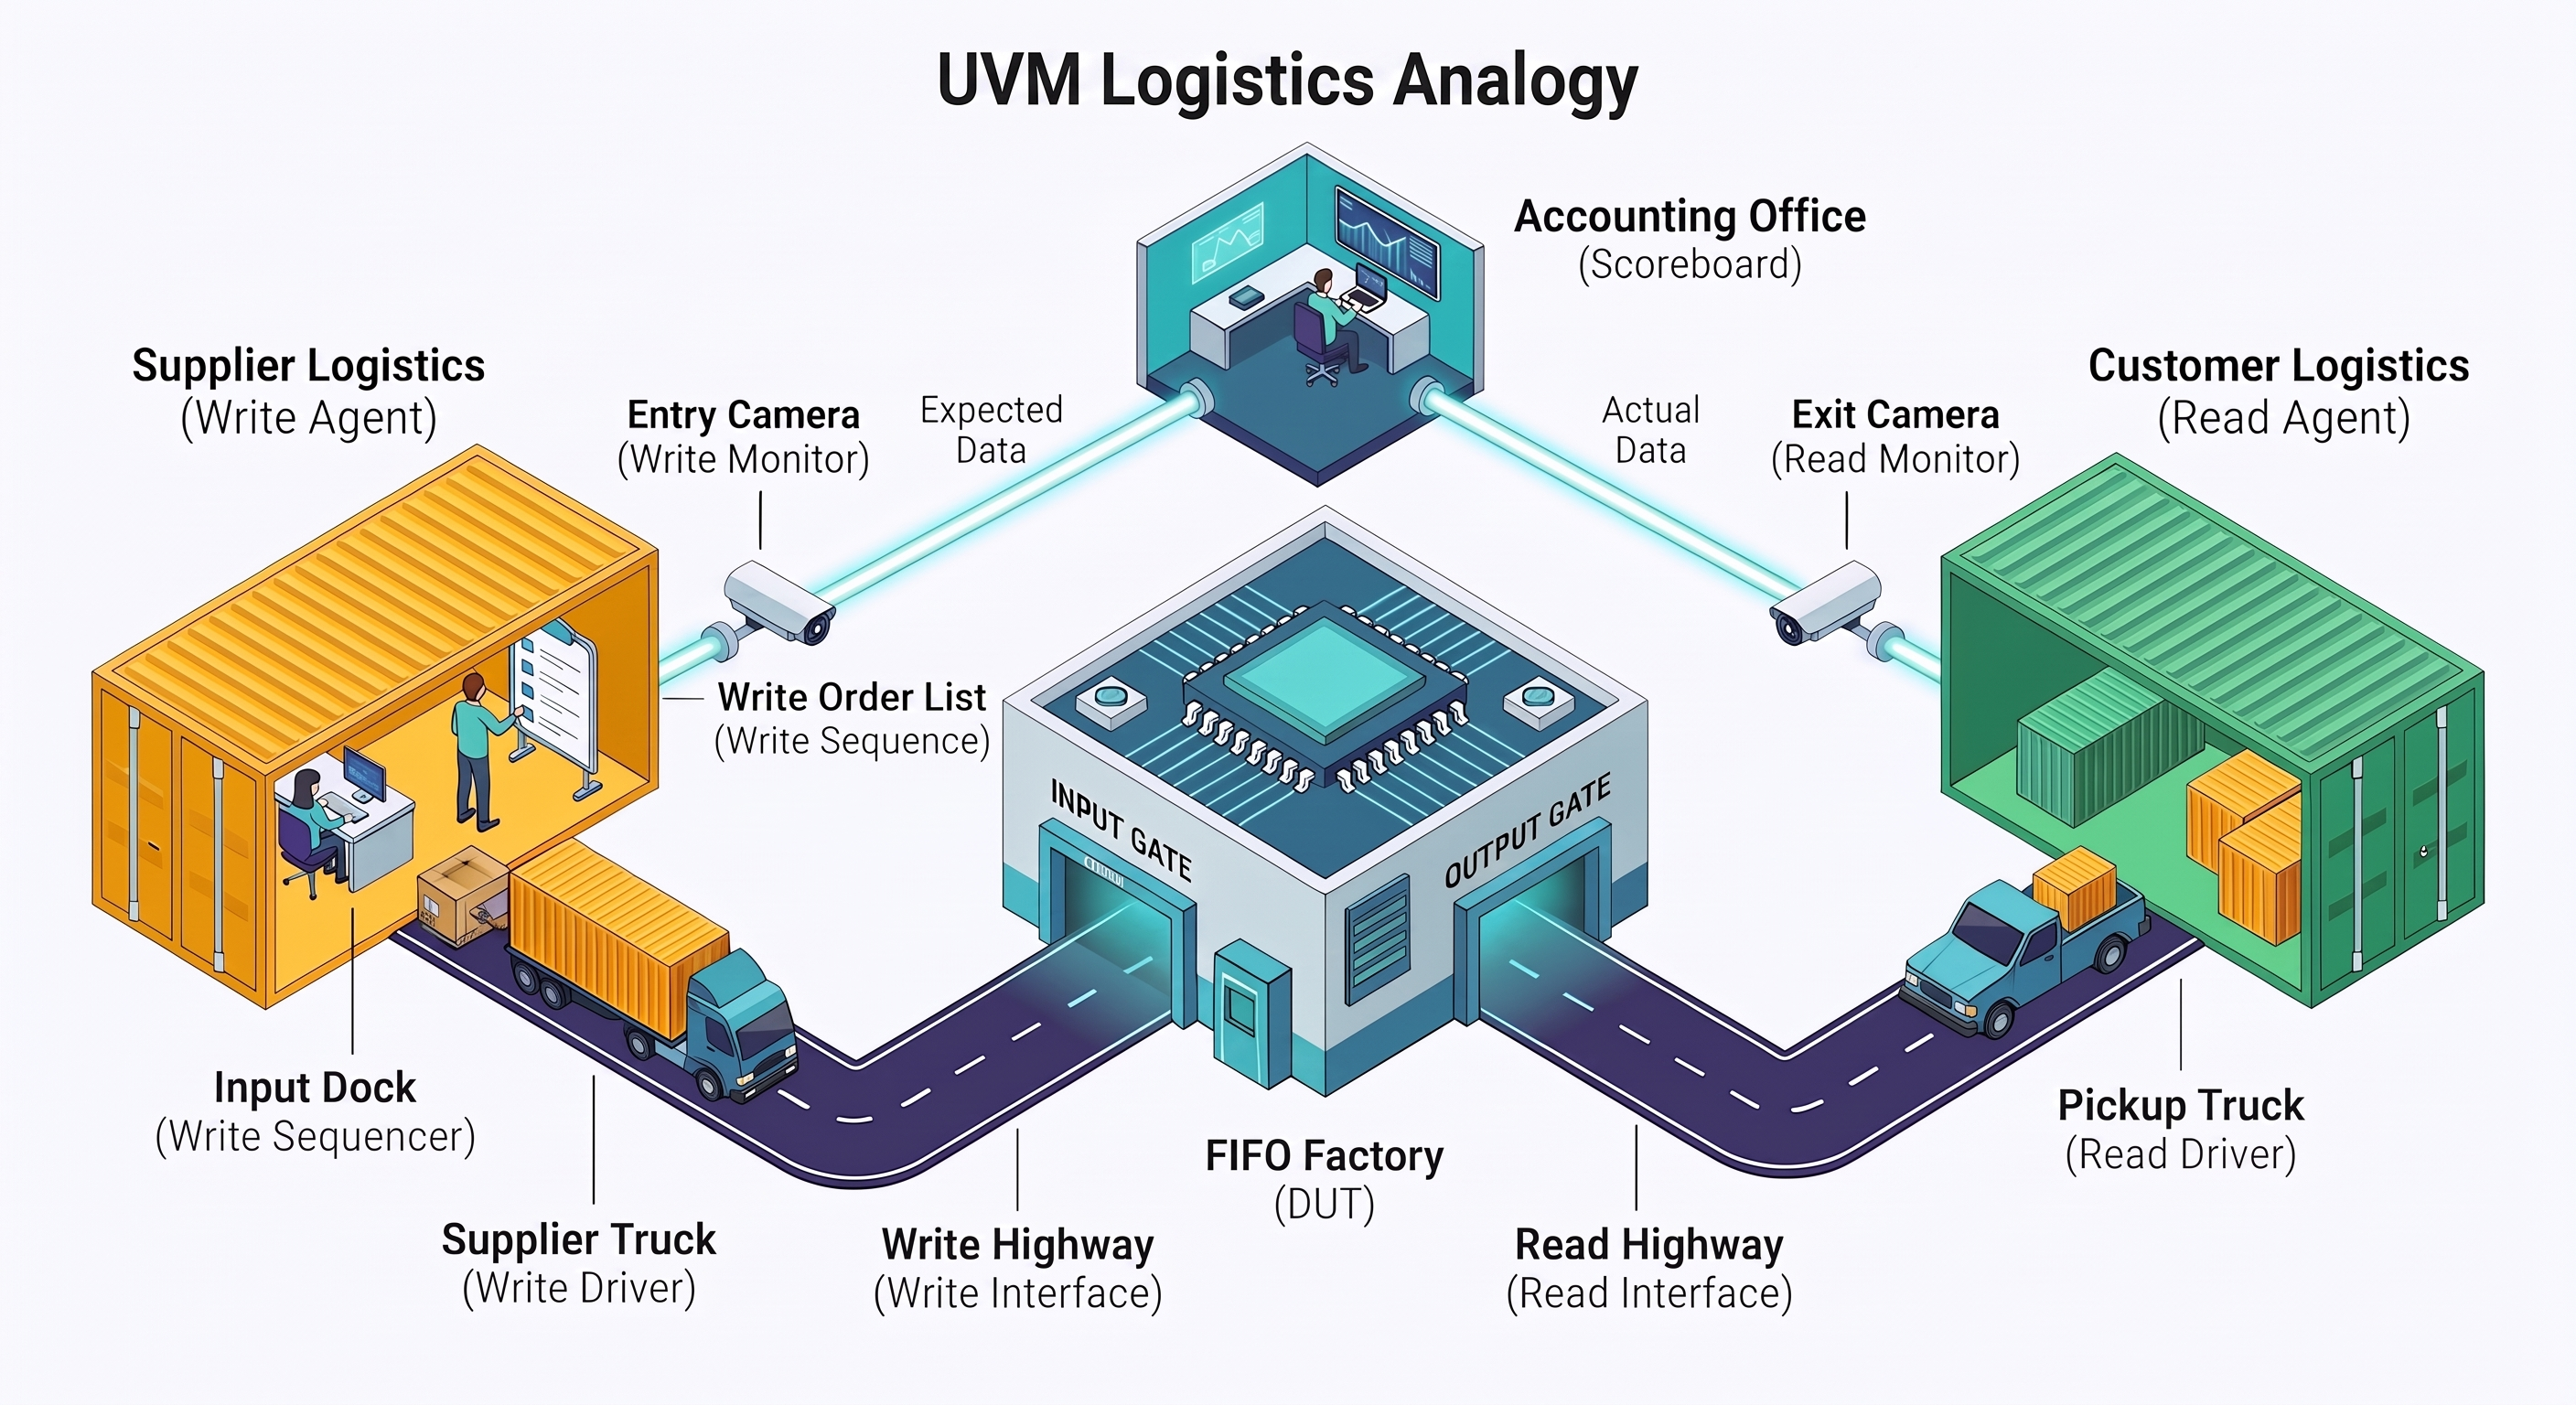
\includegraphics[keepaspectratio,alt={UVM Logistics Analogy}]{docs/uvm_logistics_analogy.jpg}}

Beyond these five primary components, the testbench relies on several
smaller elements like sequences and transactions to function. Below is
an explanation of how these parts work together to verify the FIFO,
using a shipping container logistics analogy:

{\def\LTcaptype{none} % do not increment counter
\begin{longtable}[]{@{}p{0.28\linewidth}p{0.24\linewidth}p{0.44\linewidth}@{}}
\toprule\noalign{}
Analogy & UVM Concept & Role in FIFO Verification \\
\midrule\noalign{}
\endhead
\bottomrule\noalign{}
\endlastfoot
\textbf{[Data Packet] Write Container} & \textbf{Write Transaction} & Inbound data
payload (\texttt{wdata}) driven into the FIFO. \\
\textbf{[Data Packet] Read Container} & \textbf{Read Transaction} & Outbound data
payload (\texttt{rdata}) popped from the FIFO. \\
\textbf{[Order List] Write Order List} & \textbf{Write Sequence} & Generates
planned write traffic (e.g., burst writes until \texttt{wfull}). \\
\textbf{[Order List] Read Order List} & \textbf{Read Sequence} & Generates planned
read requests (e.g., burst reads until \texttt{rempty}). \\
\textbf{[Driver Depot] Input Dock} & \textbf{Write Sequencer} & Queues write
containers for the supplier truck. \\
\textbf{[Driver Depot] Output Dock} & \textbf{Read Sequencer} & Queues read request
triggers for the pickup truck. \\
\textbf{[Transport] Supplier Truck} & \textbf{Write Driver} & Drives write
signals (\texttt{winc}, \texttt{wdata}) onto the write interface. \\
\textbf{[Transport] Pickup Truck} & \textbf{Read Driver} & Drives read request
signals (\texttt{rinc}) onto the read interface. \\
\textbf{[Highway] Supplier Logistics} & \textbf{Write Agent} & Groups Write
Sequencer, Driver, and Monitor for the write clock domain
(\texttt{wclk}). \\
\textbf{[Local Road] Customer Logistics} & \textbf{Read Agent} & Groups Read
Sequencer, Driver, and Monitor for the read clock domain
(\texttt{rclk}). \\
\textbf{[Toll Checkpoint] Write Highway} & \textbf{Write Interface} & Write clock
domain wires (\texttt{wclk}, \texttt{wrst\_n}, \texttt{winc},
\texttt{wdata}, \texttt{wfull}). \\
\textbf{[Toll Checkpoint] Read Highway} & \textbf{Read Interface} & Read clock domain
wires (\texttt{rclk}, \texttt{rrst\_n}, \texttt{rinc}, \texttt{rdata},
\texttt{rempty}). \\
\textbf{[Audit Camera] Entry Camera} & \textbf{Write Monitor} & Scans inbound
containers entering the FIFO and sends expected logs to Accounting
Office. \\
\textbf{[Audit Camera] Exit Camera} & \textbf{Read Monitor} & Scans outbound
containers leaving the FIFO and sends actual logs to Accounting
Office. \\
\textbf{[Quality Control] Accounting Office} & \textbf{Scoreboard} & Compares Expected
(Write) vs Actual (Read) containers to verify data integrity
(\textbf{PASS/FAIL}). \\
\end{longtable}
}

\subsubsection{Testbench Signal Map}\label{testbench-signal-map}

To get into the specifics, below is a table that explains how each
hardware signal is influenced by each component in the UVM testbench.

{\def\LTcaptype{none} % do not increment counter
\begin{longtable}[]{@{}p{0.20\linewidth}p{0.22\linewidth}p{0.27\linewidth}p{0.27\linewidth}@{}}
\toprule\noalign{}
Signal & Declared In & Driven By & Sampled By \\
\midrule\noalign{}
\endhead
\bottomrule\noalign{}
\endlastfoot
\textbf{\texttt{wclk}, \texttt{rclk}} &
\href{uvm/fifo_top.sv}{\texttt{uvm/fifo\_top.sv}} &
\textbf{\texttt{fifo\_top}} (\texttt{always} statement) & DUT, Interface
Clocking Blocks \\
\textbf{\texttt{wrst\_n}, \texttt{rrst\_n}} &
\href{uvm/fifo_if.sv}{\texttt{uvm/fifo\_if.sv}} &
\textbf{\texttt{fifo\_top}} (Initial Time-0) \&
\textbf{\texttt{fifo\_test}} /
\textbf{\texttt{fifo\_reset\_recovery\_test}} (Mid-traffic reset) & DUT,
Drivers, Monitors, SVA \\
\textbf{\texttt{winc}, \texttt{wdata}} &
\href{uvm/fifo_if.sv}{\texttt{uvm/fifo\_if.sv}} &
\textbf{\texttt{fifo\_w\_driver}} & DUT, \texttt{fifo\_w\_monitor},
SVA \\
\textbf{\texttt{rinc}} & \href{uvm/fifo_if.sv}{\texttt{uvm/fifo\_if.sv}}
& \textbf{\texttt{fifo\_r\_driver}} & DUT, \texttt{fifo\_r\_monitor},
SVA \\
\textbf{\texttt{wfull}, \texttt{rempty}, \texttt{rdata}} &
\href{uvm/fifo_if.sv}{\texttt{uvm/fifo\_if.sv}} & \textbf{FIFO DUT} &
Drivers, Monitors, Scoreboard, Test cases \\
\textbf{\texttt{wclken\_wire}, \texttt{rclken\_wire}} &
\href{uvm/fifo_if.sv}{\texttt{uvm/fifo\_if.sv}} & \textbf{FIFO DUT} (via
\textbf{\texttt{fifo\_connector}} bridge) & Monitors, SVA \\
\end{longtable}
}

\begin{center}\rule{0.5\linewidth}{0.5pt}\end{center}

\section{5. SVA \& Coverage}\label{5-sva--coverage}

\pandocbounded{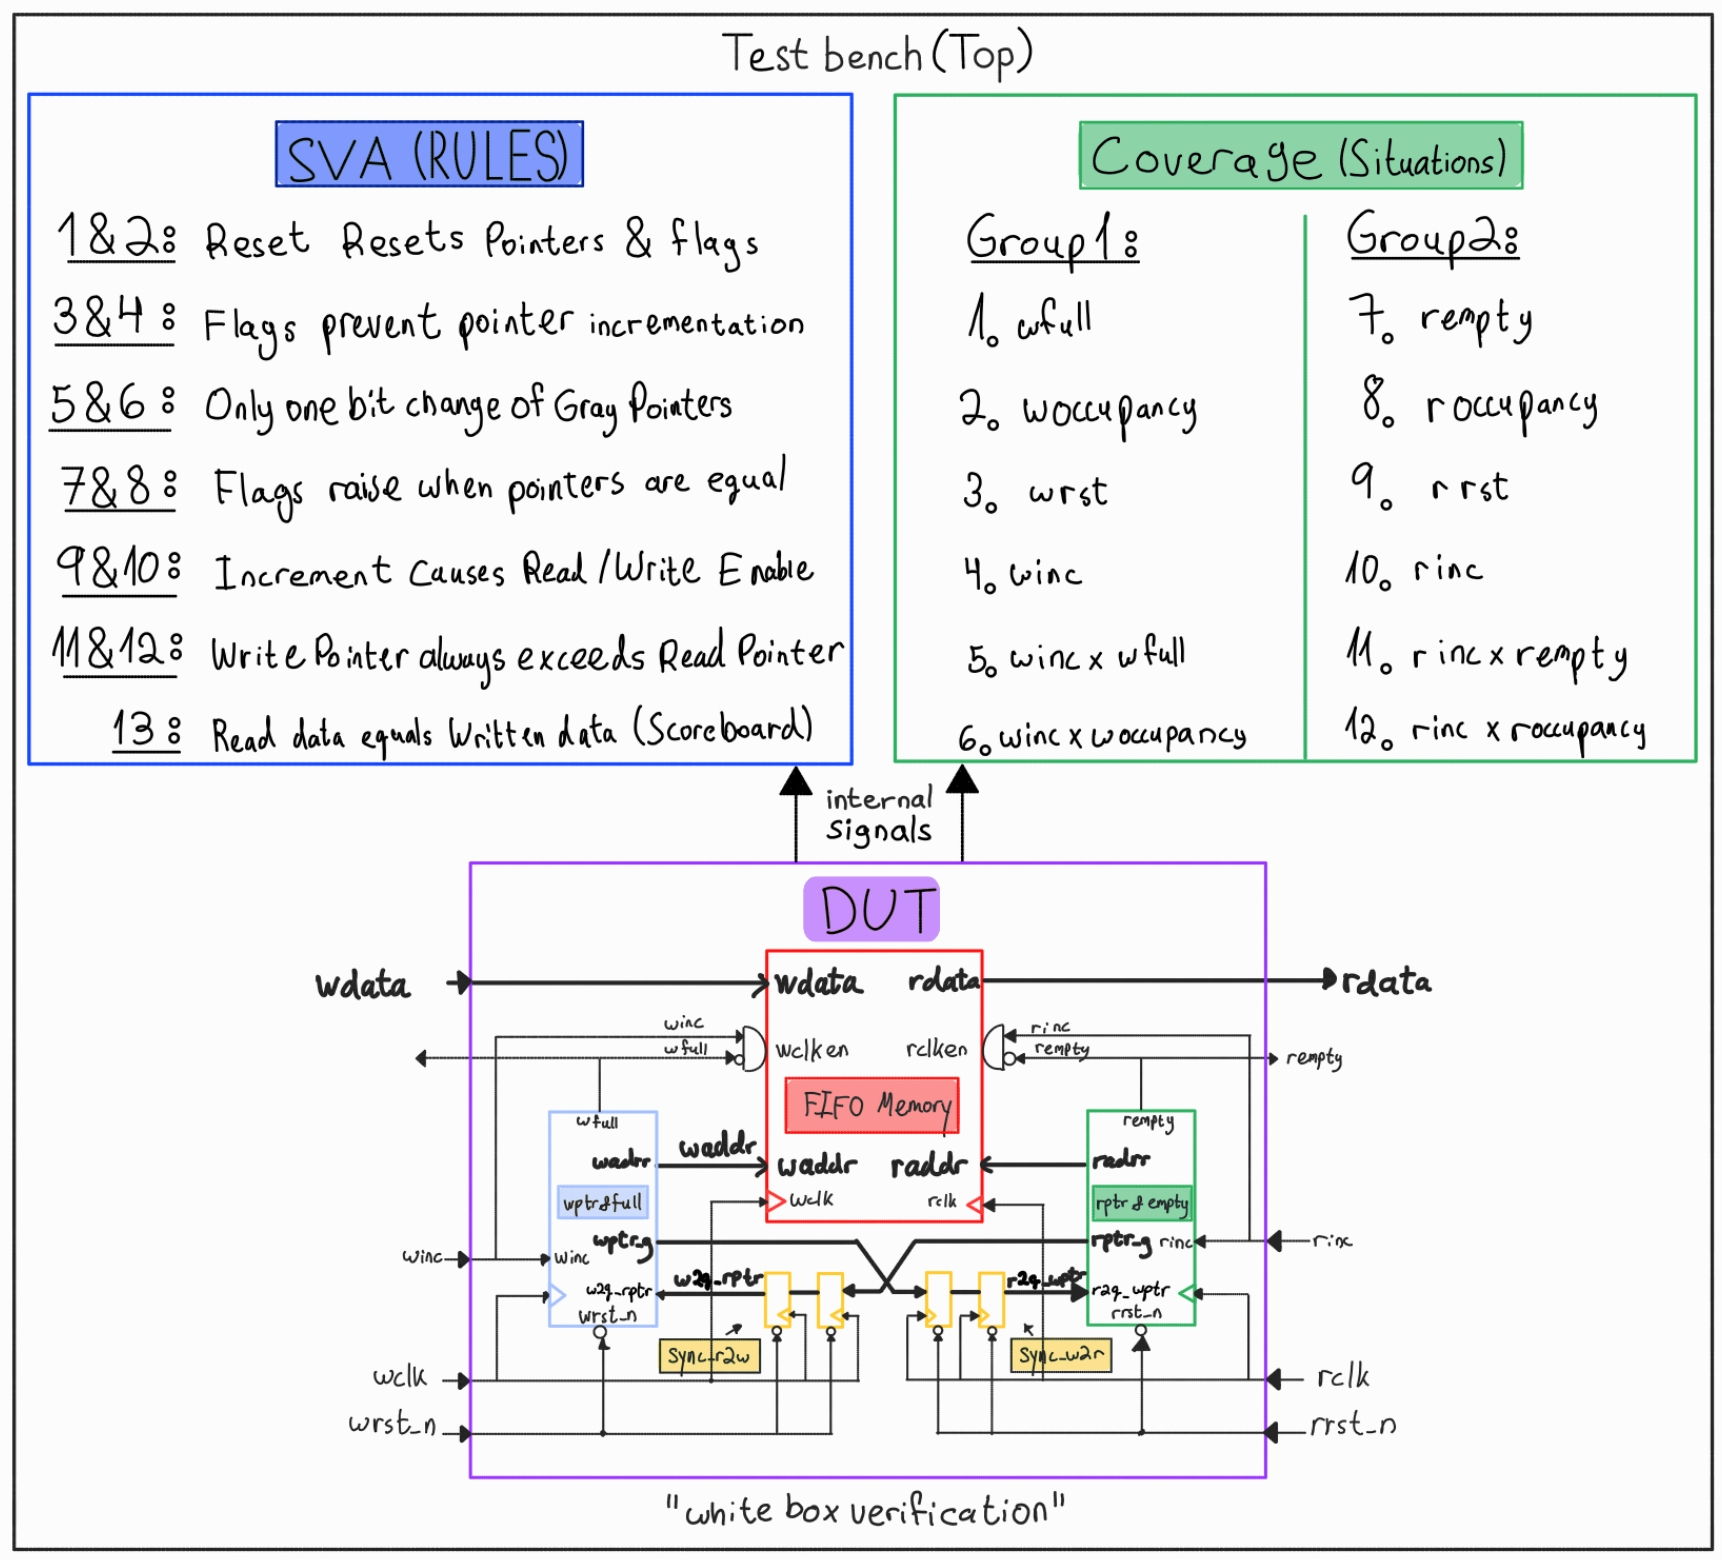
\includegraphics[keepaspectratio,alt={SVA \& Coverage Diagram}]{docs/sva_&_coverage.jpg}}

\subsection{Why use SystemVerilog
Assertions?}\label{why-use-systemverilog-assertions}

We use the \textbf{Scoreboard} as our \textbf{Black-Box} checker.
Operating in the software domain, it uses \textbf{Object-Oriented
Programming} to abstract external pin activity into high-level,
"timeless" transactions. Because it tracks abstract data rather than
physical clocks, the Scoreboard is blind to timing bugs but perfect for
verifying data that stays in the queue over long periods of time.

However, if the Scoreboard detects a failure, it only tells us that the
data broke, not \emph{why}. Did a write pointer increment too fast? Did
a synchronizer fail?

To catch these hardware-level bugs the exact cycle they happen, we
implemented \textbf{SVA} as our \textbf{White-Box} checker. Built using
strictly timed \textbf{Temporal Logic}, SVA lives in the hardware
domain. Unlike the Scoreboard, SVA is perfect for checking immediate,
short-term events. It monitors internal signals cycle-by-cycle, telling
us exactly \emph{why} and \emph{when} a protocol was violated.

\subsection{SystemVerilog Assertions - 13 Safety
Checkers}\label{systemverilog-assertions---13-safety-checkers}

The verification environment contains \textbf{13 concurrent and
immediate SystemVerilog Assertions} to check the safety and correctness
of the FIFO protocol:

\begin{enumerate}
\def\labelenumi{\arabic{enumi}.}
\tightlist
\item
  \textbf{Write Domain Reset:} Asserts that when the write reset is
  active, all write pointers (\texttt{waddr}, binary, Gray) and the full
  flag are correctly initialized to \texttt{0}.
\item
  \textbf{Read Domain Reset:} Asserts that when the read reset is
  active, all read pointers (\texttt{raddr}, binary, Gray) are
  initialized to \texttt{0} and the empty flag is asserted (\texttt{1}).
\item
  \textbf{Write Pointer Stability (No Overwrite):} Verifies that if the
  full flag is asserted, any subsequent write requests (\texttt{winc})
  will not increment the write pointers.
\item
  \textbf{Read Pointer Stability (No Overread):} Verifies that if the
  empty flag is asserted, any subsequent read requests (\texttt{rinc})
  will not increment the read pointers.
\item
  \textbf{Write Gray-Code Integrity:} Checks that the write Gray-code
  pointer changes by only one bit per increment step.
\item
  \textbf{Read Gray-Code Integrity:} Checks that the read Gray-code
  pointer changes by only one bit per increment step.
\item
  \textbf{Empty Flag Generation:} Verifies that when the read Gray
  pointer equals the synchronized write Gray pointer, the empty flag is
  asserted.
\item
  \textbf{Full Flag Generation:} Verifies that when the write Gray
  pointer matches the synchronized read Gray pointer (with the two MSBs
  inverted), the full flag is asserted.
\item
  \textbf{Write Enable Gating:} Verifies that \texttt{wclken} is only
  active when \texttt{winc\ =\ 1} and \texttt{wfull\ =\ 0}.
\item
  \textbf{Read Enable Gating:} Verifies that \texttt{rclken} is only
  active when \texttt{rinc\ =\ 1} and \texttt{rempty\ =\ 0}.
\item
  \textbf{Write Memory Occupancy Bound Check:} Verifies that the
  difference between the write pointer and synchronized read pointer
  never exceeds the FIFO depth.
\item
  \textbf{Read Memory Occupancy Bound Check:} Verifies that the
  difference between the synchronized write pointer and read pointer
  never exceeds the FIFO depth on the read side.
\item
  \textbf{Data Integrity Checker:} Compares the read data against a
  golden shadow memory array (\texttt{fifo\_data}) at the read address
  to check for data corruption.
\end{enumerate}

\subsubsection{Defense in Depth (Data
Integrity)}\label{defense-in-depth-data-integrity}

While SVA checker \#13 behaves like a scoreboard by verifying data
integrity, keeping both provides \textbf{Defense in Depth} for
debugging.

\textbf{Why check data integrity twice?} If both the SVA and the
Scoreboard fail, the internal memory array corrupted the data. If
\emph{only} the Scoreboard fails, the memory is fine, but data was
corrupted externally on the bus.

\begin{center}\rule{0.5\linewidth}{0.5pt}\end{center}

\subsection{Functional \& Structural Code
Coverage}\label{functional--structural-code-coverage}

The verification environment combines \textbf{Structural Code Coverage}
on the RTL design units with \textbf{Functional and Assertion Coverage}
defined via SystemVerilog covergroups and SVA.

\subsection{Coverage Goals \&
Coverpoints}\label{coverage-goals--coverpoints}

The verification plan defines \textbf{12 distinct coverpoints and
crosses} (split between the write-side and read-side covergroups) to
verify correct operation across all FIFO scenarios:

\subsubsection{\texorpdfstring{Write-Side Covergroup
(\texttt{fifo\_w\_cg})}{Write-Side Covergroup (fifo\_w\_cg)}}\label{write-side-covergroup-fifo_w_cg}

\begin{enumerate}
\def\labelenumi{\arabic{enumi}.}
\tightlist
\item
  \textbf{\texttt{wfull}}: Coverage of the FIFO Full flag states
  (Asserted vs. Deasserted).
\item
  \textbf{\texttt{w\_occupancy}}: Tracks write-side occupancy levels
  (\texttt{empty}, \texttt{almost\_empty}, \texttt{mid\_range},
  \texttt{almost\_full}, \texttt{full}).
\item
  \textbf{\texttt{winc}}: Verifies write command request activation.
\item
  \textbf{\texttt{wrst\_n}}: Verifies write domain reset states.
\item
  \textbf{Cross \texttt{winc} $\times$ \texttt{wfull}}: Proves write attempts
  are simulated under both Full and Non-Full conditions (tests overflow
  protection).
\item
  \textbf{Cross \texttt{winc} $\times$ \texttt{w\_occupancy}}: Proves write
  requests are executed at every possible FIFO fill level.
\end{enumerate}

\subsubsection{\texorpdfstring{Read-Side Covergroup
(\texttt{fifo\_r\_cg})}{Read-Side Covergroup (fifo\_r\_cg)}}\label{read-side-covergroup-fifo_r_cg}

\begin{enumerate}
\def\labelenumi{\arabic{enumi}.}
\setcounter{enumi}{6}
\tightlist
\item
  \textbf{\texttt{rempty}}: Coverage of the FIFO Empty flag states
  (Asserted vs. Deasserted).
\item
  \textbf{\texttt{r\_occupancy}}: Tracks read-side occupancy levels
  (\texttt{empty}, \texttt{almost\_empty}, \texttt{mid\_range},
  \texttt{almost\_full}, \texttt{full}).
\item
  \textbf{\texttt{rinc}}: Verifies read command request activation.
\item
  \textbf{\texttt{rrst\_n}}: Verifies read domain reset states.
\item
  \textbf{Cross \texttt{rinc} $\times$ \texttt{rempty}}: Proves read attempts
  are simulated under both Empty and Non-Empty conditions (tests
  underflow protection).
\item
  \textbf{Cross \texttt{rinc} $\times$ \texttt{r\_occupancy}}: Proves read
  requests are executed at every possible FIFO fill level.
\end{enumerate}

\subsection{Verification Trace Matrix (Features
Verified)}\label{verification-trace-matrix-features-verified}

{\def\LTcaptype{none} % do not increment counter
\begin{longtable}[]{@{}p{0.24\linewidth}p{0.14\linewidth}p{0.31\linewidth}p{0.27\linewidth}@{}}
\toprule\noalign{}
Verification Scenario & Status & SVA Checker Evidence & Functional
Coverage Evidence \\
\midrule\noalign{}
\endhead
\bottomrule\noalign{}
\endlastfoot
\textbf{Reset Recovery} & $\checkmark$ Passed & SVA \#1, \#2 (Write/Read Domain
Reset) & Coverpoints \texttt{wrst\_n} / \texttt{rrst\_n} \\
\textbf{Pointer Stability (Overflow/Underflow)} & $\checkmark$ Passed & SVA \#3,
\#4 (Write/Read Pointer Stability) & Crosses \texttt{winc} $\times$
\texttt{wfull} / \texttt{rinc} $\times$ \texttt{rempty} \\
\textbf{Gray Pointer Correctness} & $\checkmark$ Passed & SVA \#5, \#6 (Gray-Code
Integrity) & Indirectly by Coverpoints \texttt{w\_occupancy} /
\texttt{r\_occupancy} \\
\textbf{FIFO Flag Detection (Empty/Full)} & $\checkmark$ Passed & SVA \#7, \#8
(Flag Generation \& CDC Sync) & Coverpoints \texttt{rempty} /
\texttt{wfull} \\
\textbf{Enable Logic Gating} & $\checkmark$ Passed & SVA \#9, \#10 (Write/Read
Enable Gating) & Crosses \texttt{winc} $\times$ \texttt{wfull} / \texttt{rinc}
$\times$ \texttt{rempty} \\
\textbf{Pointer Wraparound \& Bounds} & $\checkmark$ Passed & SVA \#11, \#12
(Memory Occupancy Bound Checks) & Coverpoints \texttt{w\_occupancy} /
\texttt{r\_occupancy} \\
\textbf{Data Integrity} & $\checkmark$ Passed & SVA \#13 (Data Integrity Checker)
& Verified by UVM Scoreboard \\
\end{longtable}
}

\begin{center}\rule{0.5\linewidth}{0.5pt}\end{center}

\subsection{Coverage Results}\label{coverage-results}

{\def\LTcaptype{none} % do not increment counter
\begin{longtable}[]{@{}p{0.28\linewidth}p{0.32\linewidth}p{0.18\linewidth}p{0.16\linewidth}@{}}
\toprule\noalign{}
Coverage Type & Target & Status & Result \\
\midrule\noalign{}
\endhead
\bottomrule\noalign{}
\endlastfoot
\textbf{Functional Coverage} & Covergroups / Coverpoints & $\checkmark$ Covered &
100\% \\
\textbf{Assertion Coverage} & SystemVerilog Assertions & $\checkmark$ Covered &
100\% \\
\textbf{RTL Code Coverage} & VHDL Design Units & $\checkmark$ Covered & 100\% \\
\end{longtable}
}

\begin{itemize}
\tightlist
\item
  \textbf{Functional Coverage:} Proves the testbench successfully hit
  all defined design features and edge cases (e.g., full, empty, write
  while full).
\item
  \textbf{Assertion Coverage:} Confirms all safety checkers (SVA)
  protecting against overflow, underflow, and logic faults were active
  and passed.
\item
  \textbf{RTL Code Coverage (Structural):} Verifies the simulator
  executed every physical line, branch path, boolean expression, and
  signal toggle in the hardware code.
\end{itemize}

\subsubsection{ModelSim Coverage
Dashboard}\label{modelsim-coverage-dashboard}

\pandocbounded{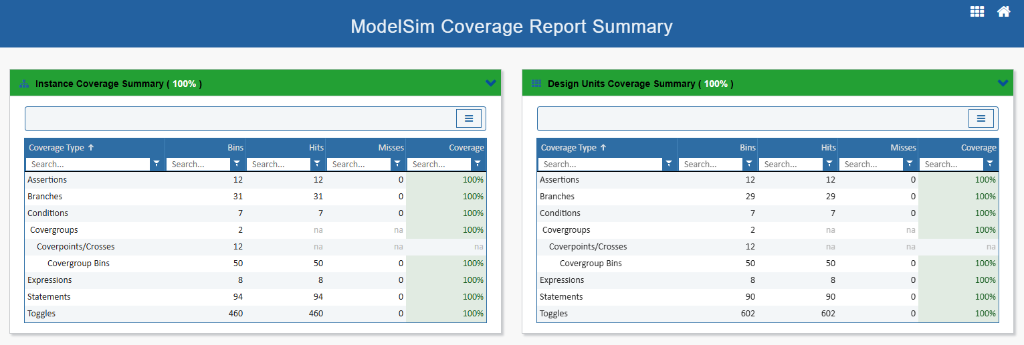
\includegraphics[keepaspectratio,alt={Coverage Report Summary}]{docs/coverage.png}}

\subsubsection{Detailed Design Units Coverage
Breakdown}\label{detailed-design-units-coverage-breakdown}

\pandocbounded{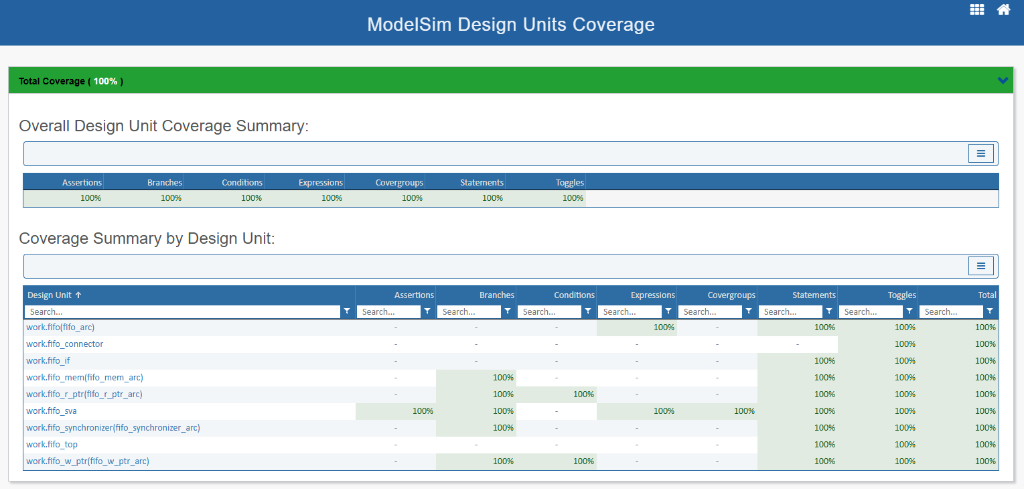
\includegraphics[keepaspectratio,alt={Detailed Design Units Coverage}]{docs/coverage_details.png}}

\begin{center}\rule{0.5\linewidth}{0.5pt}\end{center}

\section{6. Waveform Analysis \& Simulation
Guide}\label{6-waveform-analysis--simulation-guide}

\pandocbounded{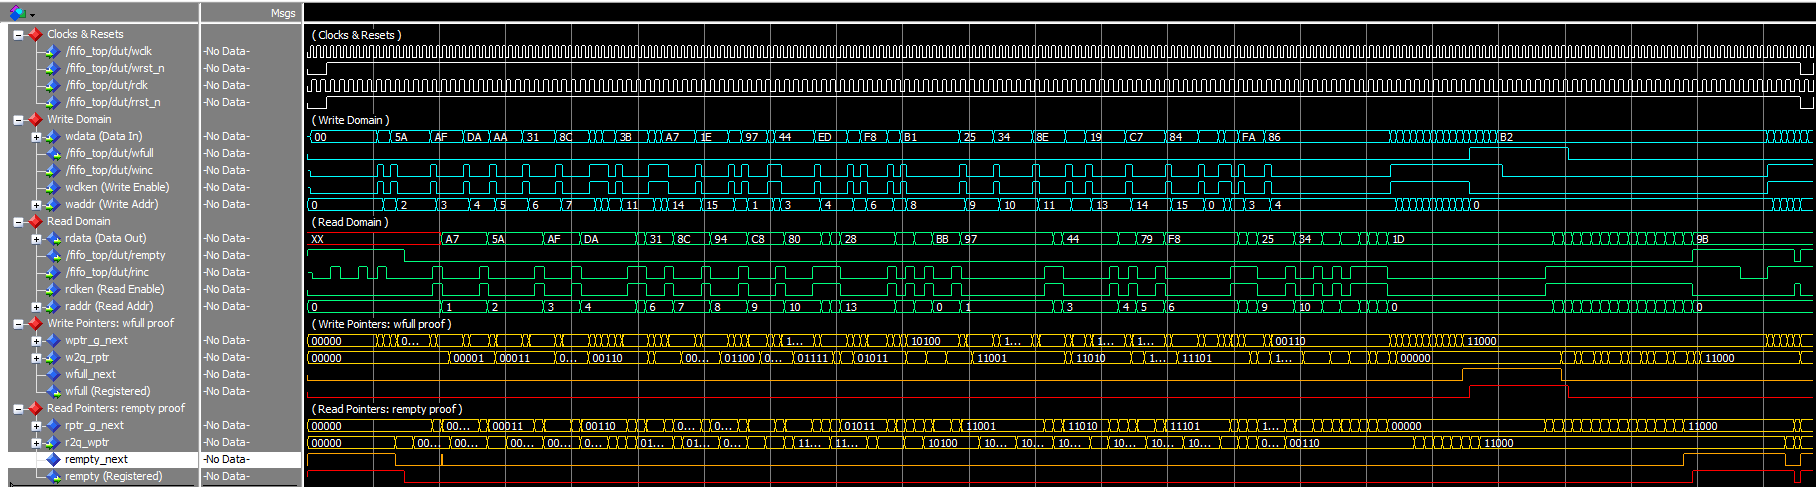
\includegraphics[keepaspectratio,alt={Waveform Simulation}]{docs/Waveform_Simulation.png}}

\section{Waveforms Colors Match Diagram
Signals}\label{waveforms-colors-match-diagram-signals}

\pandocbounded{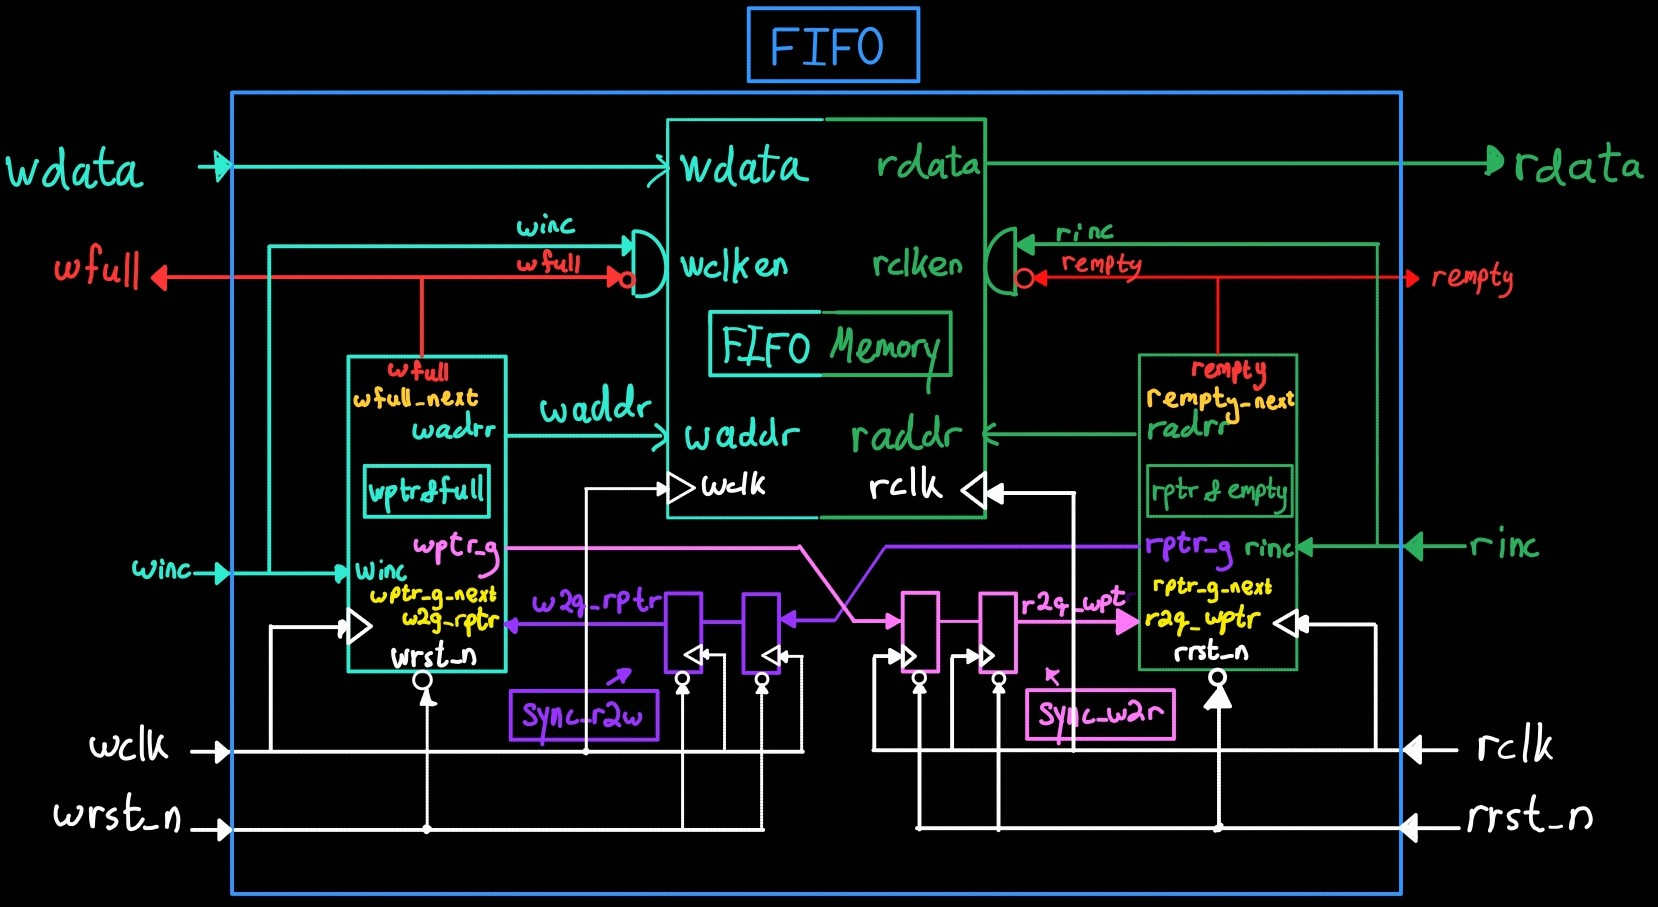
\includegraphics[keepaspectratio,alt={FIFO Block Diagram}]{docs/FIFO_Block_Diagram_Black.jpg}}

\begin{center}\rule{0.5\linewidth}{0.5pt}\end{center}

\subsection{Read \& Write Transactions}\label{read--write-transactions}

This waveform demonstrates standard FIFO data path operations. Data is
written into the memory array (\texttt{wdata}) on the write clock domain
when \texttt{winc} is asserted. It is subsequently read out
(\texttt{rdata}) on the read clock domain in a First-In-First-Out
sequence. The integrity of the data stream (e.g., \texttt{A7},
\texttt{5A}, \texttt{AF}) is preserved perfectly as it crosses the
asynchronous boundary.

\pandocbounded{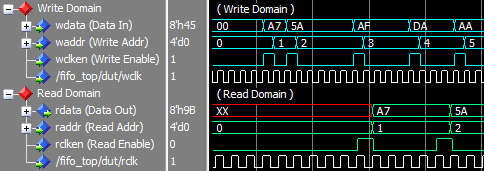
\includegraphics[keepaspectratio,alt={Read \& Write Waveform}]{docs/read_&_write_waveform.png}}

\subsubsection{2. FIFO Full Condition}\label{2-fifo-full-condition}

The FIFO asserts \texttt{wfull} when the write pointer catches up to the
synchronized read pointer. In Gray code, full occurs when pointers are
equal with the two Most Significant Bits (MSBs) inverted.

\pandocbounded{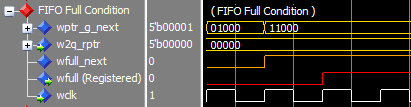
\includegraphics[keepaspectratio,alt={FIFO Full Waveform}]{docs/wfull_waveform.png}}

\subsubsection{3. FIFO Empty Condition}\label{3-fifo-empty-condition}

The FIFO asserts \texttt{rempty} when the read pointer catches up to the
synchronized write pointer (all bits match).

\pandocbounded{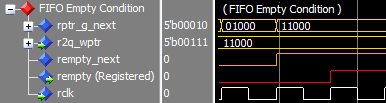
\includegraphics[keepaspectratio,alt={FIFO Empty Waveform}]{docs/rempty_waveform.png}}

\subsubsection{4. Clock Domain Crossing (CDC) Pointer
Traces}\label{4-clock-domain-crossing-cdc-pointer-traces}

\paragraph{Read-to-Write Domain
Synchronization}\label{read-to-write-domain-synchronization}

The read Gray pointer crosses into the write domain through the 2FF
synchronizer stages (\texttt{q1ptr\_g} and \texttt{q2ptr\_g}) before
being evaluated for full condition check.

\pandocbounded{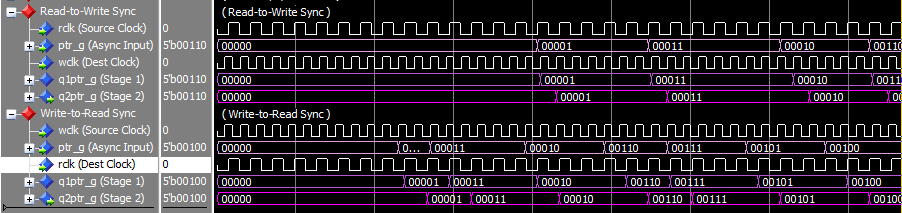
\includegraphics[keepaspectratio,alt={Read to Write Sync}]{docs/r2w_sync_waveform.png}}

\paragraph{Write-to-Read Domain
Synchronization}\label{write-to-read-domain-synchronization}

The write Gray pointer crosses into the read domain through two
flip-flop stages before empty condition evaluation.

\pandocbounded{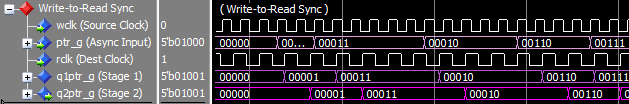
\includegraphics[keepaspectratio,alt={Write to Read Sync}]{docs/w2r_sync_waveform.png}}

\begin{center}\rule{0.5\linewidth}{0.5pt}\end{center}

\subsection{Quick Start \& Simulation
Guide}\label{quick-start--simulation-guide}

\subsubsection{Dynamic Simulation
Parameters}\label{dynamic-simulation-parameters}

You can dynamically configure \textbf{all 4 simulation parameters} at
runtime without re-compiling the design:

\subsubsection{Default Simulation
Parameters}\label{default-simulation-parameters}

\begin{itemize}
\tightlist
\item
  \textbf{Clocks:} \texttt{Wclk} = 5 ns (100 MHz), \texttt{Rclk} = 7 ns
  (\textasciitilde71.4 MHz)
\item
  \textbf{FIFO Bus:} \texttt{DataWidth} = 8 bits, \texttt{AddrWidth} = 4
  bits (\(\text{Depth} = 16\))
\end{itemize}

\begin{center}\rule{0.5\linewidth}{0.5pt}\end{center}

\subsubsection{Option 1: Automated Test Runner (Command Line - Quiet
Mode)}\label{option-1-automated-test-runner-command-line---quiet-mode}

\begin{enumerate}
\def\labelenumi{\arabic{enumi}.}
\tightlist
\item
  Open terminal and navigate to your \texttt{sim} directory:

\begin{Shaded}
\begin{Highlighting}[]
\BuiltInTok{cd}\NormalTok{ sim}
\end{Highlighting}
\end{Shaded}
\item
  Run simulation with default or custom parameters:

\begin{Shaded}
\begin{Highlighting}[]
\CommentTok{\# 1. Run basic test suite (default settings)}
\OperatorTok{.}\NormalTok{\textbackslash{}run}\OperatorTok{.}\FunctionTok{ps1}

\CommentTok{\# 2. Custom Parameters Run}
\OperatorTok{.}\NormalTok{\textbackslash{}run}\OperatorTok{.}\FunctionTok{ps1} \OperatorTok{{-}}\NormalTok{TestName fifo\_reset\_recovery\_test }\OperatorTok{{-}}\NormalTok{Wclk }\DecValTok{2} \OperatorTok{{-}}\NormalTok{Rclk }\DecValTok{10} \OperatorTok{{-}}\NormalTok{DataWidth }\DecValTok{16} \OperatorTok{{-}}\NormalTok{AddrWidth }\DecValTok{5}
\end{Highlighting}
\end{Shaded}
\end{enumerate}

\begin{center}\rule{0.5\linewidth}{0.5pt}\end{center}

\subsubsection{Option 2: Interactive ModelSim GUI
(Waveforms)}\label{option-2-interactive-modelsim-gui-waveforms}

\begin{enumerate}
\def\labelenumi{\arabic{enumi}.}
\tightlist
\item
  Open ModelSim SE and navigate to your \texttt{sim} directory:

\begin{Shaded}
\begin{Highlighting}[]
\BuiltInTok{cd}\NormalTok{ sim}
\end{Highlighting}
\end{Shaded}
\item
  Run simulation with default or custom parameters:

\begin{Shaded}
\begin{Highlighting}[]
\CommentTok{\# 1. Run basic test (default settings)}
\ControlFlowTok{do} \ExtensionTok{run.do}

\CommentTok{\# 2. Custom Parameters Run}
\BuiltInTok{set}\NormalTok{ TESTNAME fifo\_reset\_recovery\_test}\KeywordTok{;} \BuiltInTok{set}\NormalTok{ WCLK\_HALF 2}\KeywordTok{;} \BuiltInTok{set}\NormalTok{ RCLK\_HALF 10}\KeywordTok{;} \BuiltInTok{set}\NormalTok{ DATA\_WIDTH 5}\KeywordTok{;} \BuiltInTok{set}\NormalTok{ ADDR\_WIDTH 5}\KeywordTok{;} \ControlFlowTok{do} \ExtensionTok{run.do}
\end{Highlighting}
\end{Shaded}
\end{enumerate}

\begin{center}\rule{0.5\linewidth}{0.5pt}\end{center}

\subsubsection{Author}\label{author}

\textbf{Shlomo Abrams}\\
\emph{Electrical Engineering Student}\\
\href{https://github.com/ShlomoAbrams}{GitHub}

\end{document}
